


% Header, overrides base

    % Make sure that the sphinx doc style knows who it inherits from.
    \def\sphinxdocclass{article}

    % Declare the document class
    \documentclass[letterpaper,10pt,english]{/usr/local/lib/python2.7/site-packages/sphinx/texinputs/sphinxhowto}

    % Imports
    \usepackage[utf8]{inputenc}
    \DeclareUnicodeCharacter{00A0}{\\nobreakspace}
    \usepackage[T1]{fontenc}
    \usepackage{babel}
    \usepackage{times}
    \usepackage{import}
    \usepackage[Bjarne]{/usr/local/lib/python2.7/site-packages/sphinx/texinputs/fncychap}
    \usepackage{longtable}
    \usepackage{/usr/local/lib/python2.7/site-packages/sphinx/texinputs/sphinx}
    \usepackage{multirow}

    \usepackage{amsmath}
    \usepackage{amssymb}
    \usepackage{ucs}
    \usepackage{enumerate}

    % Used to make the Input/Output rules follow around the contents.
    \usepackage{needspace}
    % Pygments requirements
    \usepackage{fancyvrb}
    \usepackage{color}
    % ansi colors additions
    \definecolor{darkgreen}{rgb}{.12,.54,.11}
    \definecolor{lightgray}{gray}{.95}
    \definecolor{brown}{rgb}{0.54,0.27,0.07}
    \definecolor{purple}{rgb}{0.5,0.0,0.5}
    \definecolor{darkgray}{gray}{0.25}
    \definecolor{lightred}{rgb}{1.0,0.39,0.28}
    \definecolor{lightgreen}{rgb}{0.48,0.99,0.0}
    \definecolor{lightblue}{rgb}{0.53,0.81,0.92}
    \definecolor{lightpurple}{rgb}{0.87,0.63,0.87}
    \definecolor{lightcyan}{rgb}{0.5,1.0,0.83}

    % Needed to box output/input
    \usepackage{tikz}
        \usetikzlibrary{calc,arrows,shadows}
    \usepackage[framemethod=tikz]{mdframed}

    \usepackage{alltt}

    % Used to load and display graphics
    \usepackage{graphicx}
    \graphicspath{ {figs/} }
    \usepackage[Export]{adjustbox} % To resize


    % For formatting output while also word wrapping.
    \usepackage{listings}
    \lstset{breaklines=true}
    \lstset{basicstyle=\small\ttfamily}
    \def\smaller{\fontsize{9.5pt}{9.5pt}\selectfont}

    %Pygments definitions
    
\makeatletter
\def\PY@reset{\let\PY@it=\relax \let\PY@bf=\relax%
    \let\PY@ul=\relax \let\PY@tc=\relax%
    \let\PY@bc=\relax \let\PY@ff=\relax}
\def\PY@tok#1{\csname PY@tok@#1\endcsname}
\def\PY@toks#1+{\ifx\relax#1\empty\else%
    \PY@tok{#1}\expandafter\PY@toks\fi}
\def\PY@do#1{\PY@bc{\PY@tc{\PY@ul{%
    \PY@it{\PY@bf{\PY@ff{#1}}}}}}}
\def\PY#1#2{\PY@reset\PY@toks#1+\relax+\PY@do{#2}}

\expandafter\def\csname PY@tok@gd\endcsname{\def\PY@tc##1{\textcolor[rgb]{0.63,0.00,0.00}{##1}}}
\expandafter\def\csname PY@tok@gu\endcsname{\let\PY@bf=\textbf\def\PY@tc##1{\textcolor[rgb]{0.50,0.00,0.50}{##1}}}
\expandafter\def\csname PY@tok@gt\endcsname{\def\PY@tc##1{\textcolor[rgb]{0.00,0.27,0.87}{##1}}}
\expandafter\def\csname PY@tok@gs\endcsname{\let\PY@bf=\textbf}
\expandafter\def\csname PY@tok@gr\endcsname{\def\PY@tc##1{\textcolor[rgb]{1.00,0.00,0.00}{##1}}}
\expandafter\def\csname PY@tok@cm\endcsname{\let\PY@it=\textit\def\PY@tc##1{\textcolor[rgb]{0.25,0.50,0.50}{##1}}}
\expandafter\def\csname PY@tok@vg\endcsname{\def\PY@tc##1{\textcolor[rgb]{0.10,0.09,0.49}{##1}}}
\expandafter\def\csname PY@tok@m\endcsname{\def\PY@tc##1{\textcolor[rgb]{0.40,0.40,0.40}{##1}}}
\expandafter\def\csname PY@tok@mh\endcsname{\def\PY@tc##1{\textcolor[rgb]{0.40,0.40,0.40}{##1}}}
\expandafter\def\csname PY@tok@go\endcsname{\def\PY@tc##1{\textcolor[rgb]{0.53,0.53,0.53}{##1}}}
\expandafter\def\csname PY@tok@ge\endcsname{\let\PY@it=\textit}
\expandafter\def\csname PY@tok@vc\endcsname{\def\PY@tc##1{\textcolor[rgb]{0.10,0.09,0.49}{##1}}}
\expandafter\def\csname PY@tok@il\endcsname{\def\PY@tc##1{\textcolor[rgb]{0.40,0.40,0.40}{##1}}}
\expandafter\def\csname PY@tok@cs\endcsname{\let\PY@it=\textit\def\PY@tc##1{\textcolor[rgb]{0.25,0.50,0.50}{##1}}}
\expandafter\def\csname PY@tok@cp\endcsname{\def\PY@tc##1{\textcolor[rgb]{0.74,0.48,0.00}{##1}}}
\expandafter\def\csname PY@tok@gi\endcsname{\def\PY@tc##1{\textcolor[rgb]{0.00,0.63,0.00}{##1}}}
\expandafter\def\csname PY@tok@gh\endcsname{\let\PY@bf=\textbf\def\PY@tc##1{\textcolor[rgb]{0.00,0.00,0.50}{##1}}}
\expandafter\def\csname PY@tok@ni\endcsname{\let\PY@bf=\textbf\def\PY@tc##1{\textcolor[rgb]{0.60,0.60,0.60}{##1}}}
\expandafter\def\csname PY@tok@nl\endcsname{\def\PY@tc##1{\textcolor[rgb]{0.63,0.63,0.00}{##1}}}
\expandafter\def\csname PY@tok@nn\endcsname{\let\PY@bf=\textbf\def\PY@tc##1{\textcolor[rgb]{0.00,0.00,1.00}{##1}}}
\expandafter\def\csname PY@tok@no\endcsname{\def\PY@tc##1{\textcolor[rgb]{0.53,0.00,0.00}{##1}}}
\expandafter\def\csname PY@tok@na\endcsname{\def\PY@tc##1{\textcolor[rgb]{0.49,0.56,0.16}{##1}}}
\expandafter\def\csname PY@tok@nb\endcsname{\def\PY@tc##1{\textcolor[rgb]{0.00,0.50,0.00}{##1}}}
\expandafter\def\csname PY@tok@nc\endcsname{\let\PY@bf=\textbf\def\PY@tc##1{\textcolor[rgb]{0.00,0.00,1.00}{##1}}}
\expandafter\def\csname PY@tok@nd\endcsname{\def\PY@tc##1{\textcolor[rgb]{0.67,0.13,1.00}{##1}}}
\expandafter\def\csname PY@tok@ne\endcsname{\let\PY@bf=\textbf\def\PY@tc##1{\textcolor[rgb]{0.82,0.25,0.23}{##1}}}
\expandafter\def\csname PY@tok@nf\endcsname{\def\PY@tc##1{\textcolor[rgb]{0.00,0.00,1.00}{##1}}}
\expandafter\def\csname PY@tok@si\endcsname{\let\PY@bf=\textbf\def\PY@tc##1{\textcolor[rgb]{0.73,0.40,0.53}{##1}}}
\expandafter\def\csname PY@tok@s2\endcsname{\def\PY@tc##1{\textcolor[rgb]{0.73,0.13,0.13}{##1}}}
\expandafter\def\csname PY@tok@vi\endcsname{\def\PY@tc##1{\textcolor[rgb]{0.10,0.09,0.49}{##1}}}
\expandafter\def\csname PY@tok@nt\endcsname{\let\PY@bf=\textbf\def\PY@tc##1{\textcolor[rgb]{0.00,0.50,0.00}{##1}}}
\expandafter\def\csname PY@tok@nv\endcsname{\def\PY@tc##1{\textcolor[rgb]{0.10,0.09,0.49}{##1}}}
\expandafter\def\csname PY@tok@s1\endcsname{\def\PY@tc##1{\textcolor[rgb]{0.73,0.13,0.13}{##1}}}
\expandafter\def\csname PY@tok@sh\endcsname{\def\PY@tc##1{\textcolor[rgb]{0.73,0.13,0.13}{##1}}}
\expandafter\def\csname PY@tok@sc\endcsname{\def\PY@tc##1{\textcolor[rgb]{0.73,0.13,0.13}{##1}}}
\expandafter\def\csname PY@tok@sx\endcsname{\def\PY@tc##1{\textcolor[rgb]{0.00,0.50,0.00}{##1}}}
\expandafter\def\csname PY@tok@bp\endcsname{\def\PY@tc##1{\textcolor[rgb]{0.00,0.50,0.00}{##1}}}
\expandafter\def\csname PY@tok@c1\endcsname{\let\PY@it=\textit\def\PY@tc##1{\textcolor[rgb]{0.25,0.50,0.50}{##1}}}
\expandafter\def\csname PY@tok@kc\endcsname{\let\PY@bf=\textbf\def\PY@tc##1{\textcolor[rgb]{0.00,0.50,0.00}{##1}}}
\expandafter\def\csname PY@tok@c\endcsname{\let\PY@it=\textit\def\PY@tc##1{\textcolor[rgb]{0.25,0.50,0.50}{##1}}}
\expandafter\def\csname PY@tok@mf\endcsname{\def\PY@tc##1{\textcolor[rgb]{0.40,0.40,0.40}{##1}}}
\expandafter\def\csname PY@tok@err\endcsname{\def\PY@bc##1{\setlength{\fboxsep}{0pt}\fcolorbox[rgb]{1.00,0.00,0.00}{1,1,1}{\strut ##1}}}
\expandafter\def\csname PY@tok@kd\endcsname{\let\PY@bf=\textbf\def\PY@tc##1{\textcolor[rgb]{0.00,0.50,0.00}{##1}}}
\expandafter\def\csname PY@tok@ss\endcsname{\def\PY@tc##1{\textcolor[rgb]{0.10,0.09,0.49}{##1}}}
\expandafter\def\csname PY@tok@sr\endcsname{\def\PY@tc##1{\textcolor[rgb]{0.73,0.40,0.53}{##1}}}
\expandafter\def\csname PY@tok@mo\endcsname{\def\PY@tc##1{\textcolor[rgb]{0.40,0.40,0.40}{##1}}}
\expandafter\def\csname PY@tok@kn\endcsname{\let\PY@bf=\textbf\def\PY@tc##1{\textcolor[rgb]{0.00,0.50,0.00}{##1}}}
\expandafter\def\csname PY@tok@mi\endcsname{\def\PY@tc##1{\textcolor[rgb]{0.40,0.40,0.40}{##1}}}
\expandafter\def\csname PY@tok@gp\endcsname{\let\PY@bf=\textbf\def\PY@tc##1{\textcolor[rgb]{0.00,0.00,0.50}{##1}}}
\expandafter\def\csname PY@tok@o\endcsname{\def\PY@tc##1{\textcolor[rgb]{0.40,0.40,0.40}{##1}}}
\expandafter\def\csname PY@tok@kr\endcsname{\let\PY@bf=\textbf\def\PY@tc##1{\textcolor[rgb]{0.00,0.50,0.00}{##1}}}
\expandafter\def\csname PY@tok@s\endcsname{\def\PY@tc##1{\textcolor[rgb]{0.73,0.13,0.13}{##1}}}
\expandafter\def\csname PY@tok@kp\endcsname{\def\PY@tc##1{\textcolor[rgb]{0.00,0.50,0.00}{##1}}}
\expandafter\def\csname PY@tok@w\endcsname{\def\PY@tc##1{\textcolor[rgb]{0.73,0.73,0.73}{##1}}}
\expandafter\def\csname PY@tok@kt\endcsname{\def\PY@tc##1{\textcolor[rgb]{0.69,0.00,0.25}{##1}}}
\expandafter\def\csname PY@tok@ow\endcsname{\let\PY@bf=\textbf\def\PY@tc##1{\textcolor[rgb]{0.67,0.13,1.00}{##1}}}
\expandafter\def\csname PY@tok@sb\endcsname{\def\PY@tc##1{\textcolor[rgb]{0.73,0.13,0.13}{##1}}}
\expandafter\def\csname PY@tok@k\endcsname{\let\PY@bf=\textbf\def\PY@tc##1{\textcolor[rgb]{0.00,0.50,0.00}{##1}}}
\expandafter\def\csname PY@tok@se\endcsname{\let\PY@bf=\textbf\def\PY@tc##1{\textcolor[rgb]{0.73,0.40,0.13}{##1}}}
\expandafter\def\csname PY@tok@sd\endcsname{\let\PY@it=\textit\def\PY@tc##1{\textcolor[rgb]{0.73,0.13,0.13}{##1}}}

\def\PYZbs{\char`\\}
\def\PYZus{\char`\_}
\def\PYZob{\char`\{}
\def\PYZcb{\char`\}}
\def\PYZca{\char`\^}
\def\PYZam{\char`\&}
\def\PYZlt{\char`\<}
\def\PYZgt{\char`\>}
\def\PYZsh{\char`\#}
\def\PYZpc{\char`\%}
\def\PYZdl{\char`\$}
\def\PYZhy{\char`\-}
\def\PYZsq{\char`\'}
\def\PYZdq{\char`\"}
\def\PYZti{\char`\~}
% for compatibility with earlier versions
\def\PYZat{@}
\def\PYZlb{[}
\def\PYZrb{]}
\makeatother


    %Set pygments styles if needed...
    
        \definecolor{nbframe-border}{rgb}{0.867,0.867,0.867}
        \definecolor{nbframe-bg}{rgb}{0.969,0.969,0.969}
        \definecolor{nbframe-in-prompt}{rgb}{0.0,0.0,0.502}
        \definecolor{nbframe-out-prompt}{rgb}{0.545,0.0,0.0}

        \newenvironment{ColorVerbatim}
        {\begin{mdframed}[%
            roundcorner=1.0pt, %
            backgroundcolor=nbframe-bg, %
            userdefinedwidth=1\linewidth, %
            leftmargin=0.1\linewidth, %
            innerleftmargin=0pt, %
            innerrightmargin=0pt, %
            linecolor=nbframe-border, %
            linewidth=1pt, %
            usetwoside=false, %
            everyline=true, %
            innerlinewidth=3pt, %
            innerlinecolor=nbframe-bg, %
            middlelinewidth=1pt, %
            middlelinecolor=nbframe-bg, %
            outerlinewidth=0.5pt, %
            outerlinecolor=nbframe-border, %
            needspace=0pt
        ]}
        {\end{mdframed}}
        
        \newenvironment{InvisibleVerbatim}
        {\begin{mdframed}[leftmargin=0.1\linewidth,innerleftmargin=3pt,innerrightmargin=3pt, userdefinedwidth=1\linewidth, linewidth=0pt, linecolor=white, usetwoside=false]}
        {\end{mdframed}}

        \renewenvironment{Verbatim}[1][\unskip]
        {\begin{alltt}\smaller}
        {\end{alltt}}
    

    % Help prevent overflowing lines due to urls and other hard-to-break 
    % entities.  This doesn't catch everything...
    \sloppy

    % Document level variables
    \title{Arnold\_cat\_map}
    \date{July 25, 2013}
    \release{}
    \author{Unknown Author}
    \renewcommand{\releasename}{}

    % TODO: Add option for the user to specify a logo for his/her export.
    \newcommand{\sphinxlogo}{}

    % Make the index page of the document.
    \makeindex

    % Import sphinx document type specifics.
     

\pdfpageattr {/Group << /S /Transparency /I true /CS /DeviceRGB>>}

% Body

    % Start of the document
    \begin{document}

        
            \maketitle
        

        


        \part{Calculating and visualising the Arnold cat map}

    % Make sure that atleast 4 lines are below the HR
    \needspace{4\baselineskip}

    
        \vspace{6pt}
        \makebox[0.1\linewidth]{\smaller\hfill\tt\color{nbframe-in-prompt}In\hspace{4pt}{[}61{]}:\hspace{4pt}}\\*
        \vspace{-2.65\baselineskip}
        \begin{ColorVerbatim}
            \vspace{-0.7\baselineskip}
            \begin{Verbatim}[commandchars=\\\{\}]
\PY{o}{\PYZpc{}}\PY{k}{install\PYZus{}ext} \PY{n}{https}\PY{p}{:}\PY{o}{/}\PY{o}{/}\PY{n}{raw}\PY{o}{.}\PY{n}{github}\PY{o}{.}\PY{n}{com}\PY{o}{/}\PY{n}{minrk}\PY{o}{/}\PY{n}{ipython\PYZus{}extensions}\PY{o}{/}\PY{n}{master}\PY{o}{/}\PY{n}{nbtoc}\PY{o}{.}\PY{n}{py}
\end{Verbatim}

            
                \vspace{-0.2\baselineskip}
            
        \end{ColorVerbatim}
    

    

        % If the first block is an image, minipage the image.  Else
        % request a certain amount of space for the input text.
        \needspace{4\baselineskip}
        
        

            % Add document contents.
            
                \begin{InvisibleVerbatim}
                \vspace{-0.5\baselineskip}
    \begin{alltt}Installed nbtoc.py. To use it, type:
  %load_ext nbtoc
\end{alltt}

            \end{InvisibleVerbatim}
            
        
    


    % Make sure that atleast 4 lines are below the HR
    \needspace{4\baselineskip}

    
        \vspace{6pt}
        \makebox[0.1\linewidth]{\smaller\hfill\tt\color{nbframe-in-prompt}In\hspace{4pt}{[}63{]}:\hspace{4pt}}\\*
        \vspace{-2.65\baselineskip}
        \begin{ColorVerbatim}
            \vspace{-0.7\baselineskip}
            \begin{Verbatim}[commandchars=\\\{\}]
\PY{o}{\PYZpc{}}\PY{k}{reload\PYZus{}ext} \PY{n}{nbtoc}
\end{Verbatim}

            
                \vspace{-0.2\baselineskip}
            
        \end{ColorVerbatim}
    


    % Make sure that atleast 4 lines are below the HR
    \needspace{4\baselineskip}

    
        \vspace{6pt}
        \makebox[0.1\linewidth]{\smaller\hfill\tt\color{nbframe-in-prompt}In\hspace{4pt}{[}64{]}:\hspace{4pt}}\\*
        \vspace{-2.65\baselineskip}
        \begin{ColorVerbatim}
            \vspace{-0.7\baselineskip}
            \begin{Verbatim}[commandchars=\\\{\}]
\PY{o}{\PYZpc{}}\PY{k}{nbtoc}
\end{Verbatim}

            
                \vspace{-0.2\baselineskip}
            
        \end{ColorVerbatim}
    

    

        % If the first block is an image, minipage the image.  Else
        % request a certain amount of space for the input text.
        \needspace{4\baselineskip}
        
        

            % Add document contents.
            
                \begin{InvisibleVerbatim}
                \vspace{-0.5\baselineskip}
            \end{InvisibleVerbatim}
            
                \begin{InvisibleVerbatim}
                \vspace{-0.5\baselineskip}
            \end{InvisibleVerbatim}
            
        
    
The Arnold cat map is a canonical example of a (uniformly)
\emph{hyperbolic} (``\emph{chaotic}'') dynamical system. In this
notebook, we will use computational geometry to construct figures
showing the action of the cat map.

    % Make sure that atleast 4 lines are below the HR
    \needspace{4\baselineskip}

    
        \vspace{6pt}
        \makebox[0.1\linewidth]{\smaller\hfill\tt\color{nbframe-in-prompt}In\hspace{4pt}{[}57{]}:\hspace{4pt}}\\*
        \vspace{-2.65\baselineskip}
        \begin{ColorVerbatim}
            \vspace{-0.7\baselineskip}
            \begin{Verbatim}[commandchars=\\\{\}]
\PY{o}{\PYZpc{}}\PY{k}{nbtoc}
\end{Verbatim}

            
                \vspace{-0.2\baselineskip}
            
        \end{ColorVerbatim}
    

    

        % If the first block is an image, minipage the image.  Else
        % request a certain amount of space for the input text.
        \needspace{4\baselineskip}
        
        

            % Add document contents.
            
                \begin{InvisibleVerbatim}
                \vspace{-0.5\baselineskip}
            \end{InvisibleVerbatim}
            
                \begin{InvisibleVerbatim}
                \vspace{-0.5\baselineskip}
            \end{InvisibleVerbatim}
            
        
    


    % Make sure that atleast 4 lines are below the HR
    \needspace{4\baselineskip}

    
        \vspace{6pt}
        \makebox[0.1\linewidth]{\smaller\hfill\tt\color{nbframe-in-prompt}In\hspace{4pt}{[}8{]}:\hspace{4pt}}\\*
        \vspace{-2.65\baselineskip}
        \begin{ColorVerbatim}
            \vspace{-0.7\baselineskip}
            \begin{Verbatim}[commandchars=\\\{\}]
\PY{k+kn}{import} \PY{n+nn}{numpy} \PY{k+kn}{as} \PY{n+nn}{np}
\end{Verbatim}

            
                \vspace{-0.2\baselineskip}
            
        \end{ColorVerbatim}
    


    % Make sure that atleast 4 lines are below the HR
    \needspace{4\baselineskip}

    
        \vspace{6pt}
        \makebox[0.1\linewidth]{\smaller\hfill\tt\color{nbframe-in-prompt}In\hspace{4pt}{[}9{]}:\hspace{4pt}}\\*
        \vspace{-2.65\baselineskip}
        \begin{ColorVerbatim}
            \vspace{-0.7\baselineskip}
            \begin{Verbatim}[commandchars=\\\{\}]
\PY{k}{def} \PY{n+nf}{norm}\PY{p}{(}\PY{n}{v}\PY{p}{)}\PY{p}{:}
    \PY{k}{return} \PY{n}{np}\PY{o}{.}\PY{n}{sqrt}\PY{p}{(}\PY{n}{np}\PY{o}{.}\PY{n}{dot}\PY{p}{(}\PY{n}{v}\PY{p}{,} \PY{n}{v}\PY{p}{)}\PY{p}{)}
\end{Verbatim}

            
                \vspace{-0.2\baselineskip}
            
        \end{ColorVerbatim}
    


    % Make sure that atleast 4 lines are below the HR
    \needspace{4\baselineskip}

    
        \vspace{6pt}
        \makebox[0.1\linewidth]{\smaller\hfill\tt\color{nbframe-in-prompt}In\hspace{4pt}{[}10{]}:\hspace{4pt}}\\*
        \vspace{-2.65\baselineskip}
        \begin{ColorVerbatim}
            \vspace{-0.7\baselineskip}
            \begin{Verbatim}[commandchars=\\\{\}]
\PY{o}{\PYZpc{}}\PY{k}{load\PYZus{}ext} \PY{n}{nbtoc}
\end{Verbatim}

            
                \vspace{-0.2\baselineskip}
            
        \end{ColorVerbatim}
    

    

        % If the first block is an image, minipage the image.  Else
        % request a certain amount of space for the input text.
        \needspace{4\baselineskip}
        
        

            % Add document contents.
            
                \begin{InvisibleVerbatim}
                \vspace{-0.5\baselineskip}
    \begin{alltt}The nbtoc extension is already loaded. To reload it, use:
  %reload_ext nbtoc
\end{alltt}

            \end{InvisibleVerbatim}
            
        
    


    % Make sure that atleast 4 lines are below the HR
    \needspace{4\baselineskip}

    
        \vspace{6pt}
        \makebox[0.1\linewidth]{\smaller\hfill\tt\color{nbframe-in-prompt}In\hspace{4pt}{[}11{]}:\hspace{4pt}}\\*
        \vspace{-2.65\baselineskip}
        \begin{ColorVerbatim}
            \vspace{-0.7\baselineskip}
            \begin{Verbatim}[commandchars=\\\{\}]
\PY{o}{\PYZpc{}}\PY{k}{nbtoc}
\end{Verbatim}

            
                \vspace{-0.2\baselineskip}
            
        \end{ColorVerbatim}
    

    

        % If the first block is an image, minipage the image.  Else
        % request a certain amount of space for the input text.
        \needspace{4\baselineskip}
        
        

            % Add document contents.
            
                \begin{InvisibleVerbatim}
                \vspace{-0.5\baselineskip}
            \end{InvisibleVerbatim}
            
                \begin{InvisibleVerbatim}
                \vspace{-0.5\baselineskip}
            \end{InvisibleVerbatim}
            
        
    
\section{Simple computational geometry}It is first necessary to do define some simple concepts and functions
from computational geometry.\subsection{Line segments}We first define an object to represent a directed line segment joining
two points $\mathbf{p}_0$ and $\mathbf{p}_1$.

    % Make sure that atleast 4 lines are below the HR
    \needspace{4\baselineskip}

    
        \vspace{6pt}
        \makebox[0.1\linewidth]{\smaller\hfill\tt\color{nbframe-in-prompt}In\hspace{4pt}{[}12{]}:\hspace{4pt}}\\*
        \vspace{-2.65\baselineskip}
        \begin{ColorVerbatim}
            \vspace{-0.7\baselineskip}
            \begin{Verbatim}[commandchars=\\\{\}]
\PY{k}{class} \PY{n+nc}{DirectedLineSegment}\PY{p}{:}
    \PY{l+s+sd}{\PYZdq{}\PYZdq{}\PYZdq{}A directed line segment from `start` to `end`}
\PY{l+s+sd}{    v is the *non\PYZhy{}normalized* vector start \PYZhy{} end}
\PY{l+s+sd}{    It is non\PYZhy{}normalized so that the segment is parametrized by start + t*v, }
\PY{l+s+sd}{    where t=0 gives start and t=1 gives end}
\PY{l+s+sd}{    }
\PY{l+s+sd}{    The normal vector n is normalized.}
\PY{l+s+sd}{    \PYZdq{}\PYZdq{}\PYZdq{}}

    \PY{k}{def} \PY{n+nf}{\PYZus{}\PYZus{}init\PYZus{}\PYZus{}}\PY{p}{(}\PY{n+nb+bp}{self}\PY{p}{,} \PY{n}{start}\PY{p}{,} \PY{n}{end}\PY{p}{)}\PY{p}{:}
        \PY{n+nb+bp}{self}\PY{o}{.}\PY{n}{start}\PY{p}{,} \PY{n+nb+bp}{self}\PY{o}{.}\PY{n}{end} \PY{o}{=} \PY{n}{np}\PY{o}{.}\PY{n}{asarray}\PY{p}{(}\PY{n}{start}\PY{p}{,} \PY{n}{dtype}\PY{o}{=}\PY{n+nb}{float}\PY{p}{)}\PY{p}{,} \PY{n}{np}\PY{o}{.}\PY{n}{asarray}\PY{p}{(}\PY{n}{end}\PY{p}{,} \PY{n}{dtype}\PY{o}{=}\PY{n+nb}{float}\PY{p}{)}
        \PY{n+nb+bp}{self}\PY{o}{.}\PY{n}{v} \PY{o}{=} \PY{n+nb+bp}{self}\PY{o}{.}\PY{n}{start} \PY{o}{\PYZhy{}} \PY{n+nb+bp}{self}\PY{o}{.}\PY{n}{end}
        
        \PY{n+nb+bp}{self}\PY{o}{.}\PY{n}{n} \PY{o}{=} \PY{n}{np}\PY{o}{.}\PY{n}{array}\PY{p}{(}\PY{p}{[}\PY{o}{\PYZhy{}}\PY{n+nb+bp}{self}\PY{o}{.}\PY{n}{v}\PY{p}{[}\PY{l+m+mi}{1}\PY{p}{]}\PY{p}{,} \PY{n+nb+bp}{self}\PY{o}{.}\PY{n}{v}\PY{p}{[}\PY{l+m+mi}{0}\PY{p}{]}\PY{p}{]}\PY{p}{)}
        \PY{n+nb+bp}{self}\PY{o}{.}\PY{n}{n} \PY{o}{/}\PY{o}{=} \PY{n}{norm}\PY{p}{(}\PY{n+nb+bp}{self}\PY{o}{.}\PY{n}{n}\PY{p}{)}
        
    \PY{k}{def} \PY{n+nf}{\PYZus{}\PYZus{}repr\PYZus{}\PYZus{}}\PY{p}{(}\PY{n+nb+bp}{self}\PY{p}{)}\PY{p}{:}
        \PY{k}{return} \PY{l+s}{\PYZdq{}}\PY{l+s}{DirectedLineSegment}\PY{l+s}{\PYZdq{}} \PY{o}{+} \PY{n+nb+bp}{self}\PY{o}{.}\PY{n}{\PYZus{}\PYZus{}str\PYZus{}\PYZus{}}\PY{p}{(}\PY{p}{)}
    \PY{k}{def} \PY{n+nf}{\PYZus{}\PYZus{}str\PYZus{}\PYZus{}}\PY{p}{(}\PY{n+nb+bp}{self}\PY{p}{)}\PY{p}{:}
        \PY{k}{return} \PY{l+s}{\PYZdq{}}\PY{l+s}{([}\PY{l+s+si}{\PYZpc{}g}\PY{l+s}{, }\PY{l+s+si}{\PYZpc{}g}\PY{l+s}{], [}\PY{l+s+si}{\PYZpc{}g}\PY{l+s}{, }\PY{l+s+si}{\PYZpc{}g}\PY{l+s}{])}\PY{l+s}{\PYZdq{}} \PY{o}{\PYZpc{}} \PY{p}{(}\PY{n+nb+bp}{self}\PY{o}{.}\PY{n}{start}\PY{p}{[}\PY{l+m+mi}{0}\PY{p}{]}\PY{p}{,} \PY{n+nb+bp}{self}\PY{o}{.}\PY{n}{start}\PY{p}{[}\PY{l+m+mi}{1}\PY{p}{]}\PY{p}{,} \PY{n+nb+bp}{self}\PY{o}{.}\PY{n}{end}\PY{p}{[}\PY{l+m+mi}{0}\PY{p}{]}\PY{p}{,} \PY{n+nb+bp}{self}\PY{o}{.}\PY{n}{end}\PY{p}{[}\PY{l+m+mi}{1}\PY{p}{]}\PY{p}{)}
\end{Verbatim}

            
                \vspace{-0.2\baselineskip}
            
        \end{ColorVerbatim}
    


    % Make sure that atleast 4 lines are below the HR
    \needspace{4\baselineskip}

    
        \vspace{6pt}
        \makebox[0.1\linewidth]{\smaller\hfill\tt\color{nbframe-in-prompt}In\hspace{4pt}{[}13{]}:\hspace{4pt}}\\*
        \vspace{-2.65\baselineskip}
        \begin{ColorVerbatim}
            \vspace{-0.7\baselineskip}
            \begin{Verbatim}[commandchars=\\\{\}]
\PY{k}{def} \PY{n+nf}{find\PYZus{}intersection\PYZus{}segments}\PY{p}{(}\PY{n}{segment1}\PY{p}{,} \PY{n}{segment2}\PY{p}{)}\PY{p}{:}
    \PY{l+s+sd}{\PYZdq{}\PYZdq{}\PYZdq{}Find intersection of two line segments}
\PY{l+s+sd}{    }
\PY{l+s+sd}{    Returns the value of t corresponding to the parametrization of segment1 at the intersection point,}
\PY{l+s+sd}{    or None if they do not intersect within the segment ends}
\PY{l+s+sd}{    }
\PY{l+s+sd}{    Use representation with normal of ls2 for simplicity}
\PY{l+s+sd}{    }
\PY{l+s+sd}{    Parametrize segment1  as  p1 + t.v}
\PY{l+s+sd}{    Use representation of segment2 as \PYZob{}x:(x\PYZhy{}c).n = 0\PYZcb{}}
\PY{l+s+sd}{    \PYZdq{}\PYZdq{}\PYZdq{}}
    
    \PY{n}{n} \PY{o}{=} \PY{n}{segment2}\PY{o}{.}\PY{n}{n}
    \PY{n}{c} \PY{o}{=} \PY{n}{segment2}\PY{o}{.}\PY{n}{start}
    
    \PY{n}{x} \PY{o}{=} \PY{n}{segment1}\PY{o}{.}\PY{n}{start}
    \PY{n}{v} \PY{o}{=} \PY{n}{segment1}\PY{o}{.}\PY{n}{v}
    
    
    \PY{n}{threshold} \PY{o}{=} \PY{l+m+mf}{1.e\PYZhy{}15}
    
    \PY{k}{if} \PY{n+nb}{abs}\PY{p}{(}\PY{n}{np}\PY{o}{.}\PY{n}{dot}\PY{p}{(}\PY{n}{v}\PY{p}{,}\PY{n}{n}\PY{p}{)}\PY{p}{)} \PY{o}{\PYZlt{}} \PY{n}{threshold}\PY{p}{:}  \PY{c}{\PYZsh{} 0: lines are parallel}
        \PY{k}{return} \PY{n+nb+bp}{None}
    
    
    \PY{n}{t\PYZus{}star} \PY{o}{=} \PY{n}{np}\PY{o}{.}\PY{n}{dot}\PY{p}{(}\PY{n}{c} \PY{o}{\PYZhy{}} \PY{n}{x}\PY{p}{,} \PY{n}{n}\PY{p}{)} \PY{o}{/} \PY{n}{np}\PY{o}{.}\PY{n}{dot}\PY{p}{(}\PY{n}{v}\PY{p}{,} \PY{n}{n}\PY{p}{)}  \PY{c}{\PYZsh{} intersection time}
    
    \PY{k}{if} \PY{l+m+mf}{0.0} \PY{o}{\PYZlt{}}\PY{o}{=} \PY{n}{t\PYZus{}star} \PY{o}{\PYZlt{}}\PY{o}{=} \PY{l+m+mf}{1.0}\PY{p}{:}
        \PY{k}{return} \PY{p}{(}\PY{n}{t\PYZus{}star}\PY{p}{,} \PY{n}{x} \PY{o}{+} \PY{n}{t\PYZus{}star} \PY{o}{*} \PY{n}{v}\PY{p}{)}
    
    \PY{k}{else}\PY{p}{:}
        \PY{k}{return} \PY{n+nb+bp}{None}
\end{Verbatim}

            
                \vspace{-0.2\baselineskip}
            
        \end{ColorVerbatim}
    


    % Make sure that atleast 4 lines are below the HR
    \needspace{4\baselineskip}

    
        \vspace{6pt}
        \makebox[0.1\linewidth]{\smaller\hfill\tt\color{nbframe-in-prompt}In\hspace{4pt}{[}14{]}:\hspace{4pt}}\\*
        \vspace{-2.65\baselineskip}
        \begin{ColorVerbatim}
            \vspace{-0.7\baselineskip}
            \begin{Verbatim}[commandchars=\\\{\}]
\PY{n}{segment} \PY{o}{=} \PY{n}{DirectedLineSegment}\PY{p}{(}\PY{n}{np}\PY{o}{.}\PY{n}{r\PYZus{}}\PY{p}{[}\PY{l+m+mi}{0}\PY{p}{,} \PY{l+m+mi}{0}\PY{p}{]}\PY{p}{,} \PY{n}{np}\PY{o}{.}\PY{n}{r\PYZus{}}\PY{p}{[}\PY{l+m+mi}{2}\PY{p}{,} \PY{l+m+mi}{2}\PY{p}{]}\PY{p}{)}    
\end{Verbatim}

            
                \vspace{-0.2\baselineskip}
            
        \end{ColorVerbatim}
    


    % Make sure that atleast 4 lines are below the HR
    \needspace{4\baselineskip}

    
        \vspace{6pt}
        \makebox[0.1\linewidth]{\smaller\hfill\tt\color{nbframe-in-prompt}In\hspace{4pt}{[}15{]}:\hspace{4pt}}\\*
        \vspace{-2.65\baselineskip}
        \begin{ColorVerbatim}
            \vspace{-0.7\baselineskip}
            \begin{Verbatim}[commandchars=\\\{\}]
\PY{n}{segment}
\end{Verbatim}

            
                \vspace{-0.2\baselineskip}
            
        \end{ColorVerbatim}
    

    

        % If the first block is an image, minipage the image.  Else
        % request a certain amount of space for the input text.
        \needspace{4\baselineskip}
        
        

            % Add document contents.
            
                \makebox[0.1\linewidth]{\smaller\hfill\tt\color{nbframe-out-prompt}Out\hspace{4pt}{[}15{]}:\hspace{4pt}}\\*
                \vspace{-2.55\baselineskip}\begin{InvisibleVerbatim}
                \vspace{-0.5\baselineskip}
    \begin{alltt}DirectedLineSegment([0, 0], [2, 2])\end{alltt}

            \end{InvisibleVerbatim}
            
        
    


    % Make sure that atleast 4 lines are below the HR
    \needspace{4\baselineskip}

    
        \vspace{6pt}
        \makebox[0.1\linewidth]{\smaller\hfill\tt\color{nbframe-in-prompt}In\hspace{4pt}{[}16{]}:\hspace{4pt}}\\*
        \vspace{-2.65\baselineskip}
        \begin{ColorVerbatim}
            \vspace{-0.7\baselineskip}
            \begin{Verbatim}[commandchars=\\\{\}]
\PY{n}{segment}\PY{o}{.}\PY{n}{v}
\end{Verbatim}

            
                \vspace{-0.2\baselineskip}
            
        \end{ColorVerbatim}
    

    

        % If the first block is an image, minipage the image.  Else
        % request a certain amount of space for the input text.
        \needspace{4\baselineskip}
        
        

            % Add document contents.
            
                \makebox[0.1\linewidth]{\smaller\hfill\tt\color{nbframe-out-prompt}Out\hspace{4pt}{[}16{]}:\hspace{4pt}}\\*
                \vspace{-2.55\baselineskip}\begin{InvisibleVerbatim}
                \vspace{-0.5\baselineskip}
    \begin{alltt}array([-2., -2.])\end{alltt}

            \end{InvisibleVerbatim}
            
        
    


    % Make sure that atleast 4 lines are below the HR
    \needspace{4\baselineskip}

    
        \vspace{6pt}
        \makebox[0.1\linewidth]{\smaller\hfill\tt\color{nbframe-in-prompt}In\hspace{4pt}{[}17{]}:\hspace{4pt}}\\*
        \vspace{-2.65\baselineskip}
        \begin{ColorVerbatim}
            \vspace{-0.7\baselineskip}
            \begin{Verbatim}[commandchars=\\\{\}]
\PY{n}{segment1} \PY{o}{=} \PY{n}{DirectedLineSegment}\PY{p}{(}\PY{p}{[}\PY{l+m+mi}{0}\PY{p}{,} \PY{l+m+mi}{0}\PY{p}{]}\PY{p}{,} \PY{p}{[}\PY{l+m+mi}{1}\PY{p}{,} \PY{l+m+mi}{1}\PY{p}{]}\PY{p}{)}
\PY{n}{segment2} \PY{o}{=} \PY{n}{DirectedLineSegment}\PY{p}{(}\PY{p}{[}\PY{l+m+mi}{3}\PY{p}{,} \PY{l+m+mi}{3}\PY{p}{]}\PY{p}{,} \PY{p}{[}\PY{l+m+mi}{4}\PY{p}{,} \PY{l+m+mi}{4}\PY{p}{]}\PY{p}{)}

\PY{k}{print} \PY{n}{find\PYZus{}intersection\PYZus{}segments}\PY{p}{(}\PY{n}{segment1}\PY{p}{,} \PY{n}{segment2}\PY{p}{)}
\end{Verbatim}

            
                \vspace{-0.2\baselineskip}
            
        \end{ColorVerbatim}
    

    

        % If the first block is an image, minipage the image.  Else
        % request a certain amount of space for the input text.
        \needspace{4\baselineskip}
        
        

            % Add document contents.
            
                \begin{InvisibleVerbatim}
                \vspace{-0.5\baselineskip}
    \begin{alltt}None
\end{alltt}

            \end{InvisibleVerbatim}
            
        
    


    % Make sure that atleast 4 lines are below the HR
    \needspace{4\baselineskip}

    
        \vspace{6pt}
        \makebox[0.1\linewidth]{\smaller\hfill\tt\color{nbframe-in-prompt}In\hspace{4pt}{[}18{]}:\hspace{4pt}}\\*
        \vspace{-2.65\baselineskip}
        \begin{ColorVerbatim}
            \vspace{-0.7\baselineskip}
            \begin{Verbatim}[commandchars=\\\{\}]
\PY{n}{segment1} \PY{o}{=} \PY{n}{DirectedLineSegment}\PY{p}{(}\PY{p}{[}\PY{l+m+mi}{0}\PY{p}{,} \PY{l+m+mi}{0}\PY{p}{]}\PY{p}{,} \PY{p}{[}\PY{l+m+mi}{1}\PY{p}{,} \PY{l+m+mi}{1}\PY{p}{]}\PY{p}{)}
\PY{n}{segment2} \PY{o}{=} \PY{n}{DirectedLineSegment}\PY{p}{(}\PY{p}{[}\PY{l+m+mi}{1}\PY{p}{,} \PY{l+m+mi}{0}\PY{p}{]}\PY{p}{,} \PY{p}{[}\PY{l+m+mi}{0}\PY{p}{,} \PY{l+m+mi}{2}\PY{p}{]}\PY{p}{)}

\PY{k}{print} \PY{n}{find\PYZus{}intersection\PYZus{}segments}\PY{p}{(}\PY{n}{segment1}\PY{p}{,} \PY{n}{segment2}\PY{p}{)}
\end{Verbatim}

            
                \vspace{-0.2\baselineskip}
            
        \end{ColorVerbatim}
    

    

        % If the first block is an image, minipage the image.  Else
        % request a certain amount of space for the input text.
        \needspace{4\baselineskip}
        
        

            % Add document contents.
            
                \begin{InvisibleVerbatim}
                \vspace{-0.5\baselineskip}
    \begin{alltt}None
\end{alltt}

            \end{InvisibleVerbatim}
            
        
    


    % Make sure that atleast 4 lines are below the HR
    \needspace{4\baselineskip}

    
        \vspace{6pt}
        \makebox[0.1\linewidth]{\smaller\hfill\tt\color{nbframe-in-prompt}In\hspace{4pt}{[}19{]}:\hspace{4pt}}\\*
        \vspace{-2.65\baselineskip}
        \begin{ColorVerbatim}
            \vspace{-0.7\baselineskip}
            \begin{Verbatim}[commandchars=\\\{\}]
\PY{k}{def} \PY{n+nf}{test\PYZus{}find\PYZus{}intersection\PYZus{}segments}\PY{p}{(}\PY{p}{)}\PY{p}{:}

    \PY{n}{segment1} \PY{o}{=} \PY{n}{DirectedLineSegment}\PY{p}{(}\PY{p}{[}\PY{l+m+mi}{0}\PY{p}{,} \PY{l+m+mi}{0}\PY{p}{]}\PY{p}{,} \PY{p}{[}\PY{l+m+mi}{1}\PY{p}{,} \PY{l+m+mi}{1}\PY{p}{]}\PY{p}{)}
    \PY{n}{segment2} \PY{o}{=} \PY{n}{DirectedLineSegment}\PY{p}{(}\PY{p}{[}\PY{l+m+mi}{0}\PY{p}{,} \PY{l+m+mi}{1}\PY{p}{]}\PY{p}{,} \PY{p}{[}\PY{l+m+mi}{1}\PY{p}{,} \PY{l+m+mi}{0}\PY{p}{]}\PY{p}{)}
    
    \PY{n}{t\PYZus{}star}\PY{p}{,} \PY{n}{intersection\PYZus{}point} \PY{o}{=} \PY{n}{find\PYZus{}intersection\PYZus{}segments}\PY{p}{(}\PY{n}{segment1}\PY{p}{,} \PY{n}{segment2}\PY{p}{)}
    \PY{k}{assert} \PY{n}{t\PYZus{}star} \PY{o}{==} \PY{l+m+mf}{0.5}
    \PY{k}{assert} \PY{n+nb}{all}\PY{p}{(}\PY{n}{intersection\PYZus{}point} \PY{o}{==} \PY{n}{np}\PY{o}{.}\PY{n}{array}\PY{p}{(}\PY{p}{[}\PY{l+m+mf}{0.5}\PY{p}{,} \PY{l+m+mf}{0.5}\PY{p}{]}\PY{p}{)}\PY{p}{)}
    
    
    \PY{c}{\PYZsh{} parallel lines:}
    \PY{n}{segment1} \PY{o}{=} \PY{n}{DirectedLineSegment}\PY{p}{(}\PY{p}{[}\PY{l+m+mi}{0}\PY{p}{,} \PY{l+m+mi}{0}\PY{p}{]}\PY{p}{,} \PY{p}{[}\PY{l+m+mi}{1}\PY{p}{,} \PY{l+m+mi}{1}\PY{p}{]}\PY{p}{)}
    \PY{n}{segment2} \PY{o}{=} \PY{n}{DirectedLineSegment}\PY{p}{(}\PY{p}{[}\PY{l+m+mi}{3}\PY{p}{,} \PY{l+m+mi}{3}\PY{p}{]}\PY{p}{,} \PY{p}{[}\PY{l+m+mi}{4}\PY{p}{,} \PY{l+m+mi}{4}\PY{p}{]}\PY{p}{)}

    \PY{k}{assert} \PY{n}{find\PYZus{}intersection\PYZus{}segments}\PY{p}{(}\PY{n}{segment1}\PY{p}{,} \PY{n}{segment2}\PY{p}{)} \PY{o}{==} \PY{n+nb+bp}{None}
    
    
    \PY{n}{segment1} \PY{o}{=} \PY{n}{DirectedLineSegment}\PY{p}{(}\PY{p}{[}\PY{l+m+mi}{0}\PY{p}{,} \PY{l+m+mi}{0}\PY{p}{]}\PY{p}{,} \PY{p}{[}\PY{l+m+mi}{1}\PY{p}{,} \PY{l+m+mi}{1}\PY{p}{]}\PY{p}{)}
    \PY{n}{segment2} \PY{o}{=} \PY{n}{DirectedLineSegment}\PY{p}{(}\PY{p}{[}\PY{l+m+mi}{1}\PY{p}{,} \PY{l+m+mi}{1}\PY{p}{]}\PY{p}{,} \PY{p}{[}\PY{l+m+mi}{1}\PY{p}{,} \PY{l+m+mi}{2}\PY{p}{]}\PY{p}{)}
    
    \PY{n}{t\PYZus{}star}\PY{p}{,} \PY{n}{intersection\PYZus{}point} \PY{o}{=} \PY{n}{find\PYZus{}intersection\PYZus{}segments}\PY{p}{(}\PY{n}{segment1}\PY{p}{,} \PY{n}{segment2}\PY{p}{)}
    \PY{k}{assert} \PY{n}{t\PYZus{}star} \PY{o}{==} \PY{l+m+mf}{1.0}
    \PY{k}{assert} \PY{n+nb}{all}\PY{p}{(}\PY{n}{intersection\PYZus{}point} \PY{o}{==} \PY{n}{np}\PY{o}{.}\PY{n}{array}\PY{p}{(}\PY{p}{[}\PY{l+m+mf}{1.0}\PY{p}{,} \PY{l+m+mf}{1.0}\PY{p}{]}\PY{p}{)}\PY{p}{)}
    
\end{Verbatim}

            
                \vspace{-0.2\baselineskip}
            
        \end{ColorVerbatim}
    
\subsection{Polygons}Next we join line segments up into directed polygons. Here we are
assuming that the polygons are closed loops, i.e.~that there is a link
from the last vertex back to the first.

    % Make sure that atleast 4 lines are below the HR
    \needspace{4\baselineskip}

    
        \vspace{6pt}
        \makebox[0.1\linewidth]{\smaller\hfill\tt\color{nbframe-in-prompt}In\hspace{4pt}{[}20{]}:\hspace{4pt}}\\*
        \vspace{-2.65\baselineskip}
        \begin{ColorVerbatim}
            \vspace{-0.7\baselineskip}
            \begin{Verbatim}[commandchars=\\\{\}]
\PY{k}{class} \PY{n+nc}{DirectedPolygon}\PY{p}{:}
    \PY{l+s+sd}{\PYZdq{}\PYZdq{}\PYZdq{}A directed polygon}
\PY{l+s+sd}{    }
\PY{l+s+sd}{    Parameters}
\PY{l+s+sd}{    ==========}
\PY{l+s+sd}{    vertices:}
\PY{l+s+sd}{        a list of vertices}
\PY{l+s+sd}{    \PYZdq{}\PYZdq{}\PYZdq{}}
        
    
    \PY{k}{def} \PY{n+nf}{\PYZus{}\PYZus{}init\PYZus{}\PYZus{}}\PY{p}{(}\PY{n+nb+bp}{self}\PY{p}{,} \PY{n}{vertices}\PY{p}{)}\PY{p}{:}
        \PY{n+nb+bp}{self}\PY{o}{.}\PY{n}{vertices} \PY{o}{=} \PY{n}{np}\PY{o}{.}\PY{n}{asarray}\PY{p}{(}\PY{n}{vertices}\PY{p}{)}
        
        \PY{n+nb+bp}{self}\PY{o}{.}\PY{n}{segments} \PY{o}{=} \PY{p}{[}\PY{p}{]}
        
        \PY{k}{for} \PY{n}{i} \PY{o+ow}{in} \PY{n+nb}{range}\PY{p}{(}\PY{n+nb}{len}\PY{p}{(}\PY{n+nb+bp}{self}\PY{o}{.}\PY{n}{vertices}\PY{p}{)}\PY{o}{\PYZhy{}}\PY{l+m+mi}{1}\PY{p}{)}\PY{p}{:}
            \PY{n+nb+bp}{self}\PY{o}{.}\PY{n}{segments}\PY{o}{.}\PY{n}{append}\PY{p}{(}\PY{n}{DirectedLineSegment}\PY{p}{(}\PY{n+nb+bp}{self}\PY{o}{.}\PY{n}{vertices}\PY{p}{[}\PY{n}{i}\PY{p}{]}\PY{p}{,} \PY{n}{vertices}\PY{p}{[}\PY{n}{i}\PY{o}{+}\PY{l+m+mi}{1}\PY{p}{]}\PY{p}{)}\PY{p}{)}
            
        \PY{n+nb+bp}{self}\PY{o}{.}\PY{n}{segments}\PY{o}{.}\PY{n}{append}\PY{p}{(}\PY{n}{DirectedLineSegment}\PY{p}{(}\PY{n}{vertices}\PY{p}{[}\PY{o}{\PYZhy{}}\PY{l+m+mi}{1}\PY{p}{]}\PY{p}{,} \PY{n}{vertices}\PY{p}{[}\PY{l+m+mi}{0}\PY{p}{]}\PY{p}{)}\PY{p}{)}

    \PY{k}{def} \PY{n+nf}{\PYZus{}\PYZus{}repr\PYZus{}\PYZus{}}\PY{p}{(}\PY{n+nb+bp}{self}\PY{p}{)}\PY{p}{:}
        \PY{k}{return} \PY{n+nb+bp}{self}\PY{o}{.}\PY{n}{segments}\PY{o}{.}\PY{n}{\PYZus{}\PYZus{}repr\PYZus{}\PYZus{}}\PY{p}{(}\PY{p}{)}
    
    \PY{k}{def} \PY{n+nf}{draw}\PY{p}{(}\PY{n+nb+bp}{self}\PY{p}{)}\PY{p}{:}
        \PY{n}{plt}\PY{o}{.}\PY{n}{fill}\PY{p}{(}\PY{n+nb+bp}{self}\PY{o}{.}\PY{n}{vertices}\PY{p}{[}\PY{p}{:}\PY{p}{,}\PY{l+m+mi}{0}\PY{p}{]}\PY{p}{,} \PY{n+nb+bp}{self}\PY{o}{.}\PY{n}{vertices}\PY{p}{[}\PY{p}{:}\PY{p}{,}\PY{l+m+mi}{1}\PY{p}{]}\PY{p}{,} \PY{n}{alpha}\PY{o}{=}\PY{l+m+mf}{0.5}\PY{p}{)}
        
\end{Verbatim}

            
                \vspace{-0.2\baselineskip}
            
        \end{ColorVerbatim}
    


    % Make sure that atleast 4 lines are below the HR
    \needspace{4\baselineskip}

    
        \vspace{6pt}
        \makebox[0.1\linewidth]{\smaller\hfill\tt\color{nbframe-in-prompt}In\hspace{4pt}{[}21{]}:\hspace{4pt}}\\*
        \vspace{-2.65\baselineskip}
        \begin{ColorVerbatim}
            \vspace{-0.7\baselineskip}
            \begin{Verbatim}[commandchars=\\\{\}]
\PY{n}{unit\PYZus{}square} \PY{o}{=} \PY{n}{DirectedPolygon}\PY{p}{(}\PY{p}{[}\PY{p}{(}\PY{l+m+mf}{0.}\PY{p}{,}\PY{l+m+mf}{0.}\PY{p}{)}\PY{p}{,} \PY{p}{(}\PY{l+m+mf}{1.}\PY{p}{,}\PY{l+m+mf}{0.}\PY{p}{)}\PY{p}{,} \PY{p}{(}\PY{l+m+mf}{1.}\PY{p}{,}\PY{l+m+mf}{1.}\PY{p}{)}\PY{p}{,} \PY{p}{(}\PY{l+m+mf}{0.}\PY{p}{,}\PY{l+m+mf}{1.}\PY{p}{)}\PY{p}{]}\PY{p}{)}
\PY{n}{unit\PYZus{}square}
\end{Verbatim}

            
                \vspace{-0.2\baselineskip}
            
        \end{ColorVerbatim}
    

    

        % If the first block is an image, minipage the image.  Else
        % request a certain amount of space for the input text.
        \needspace{4\baselineskip}
        
        

            % Add document contents.
            
                \makebox[0.1\linewidth]{\smaller\hfill\tt\color{nbframe-out-prompt}Out\hspace{4pt}{[}21{]}:\hspace{4pt}}\\*
                \vspace{-2.55\baselineskip}\begin{InvisibleVerbatim}
                \vspace{-0.5\baselineskip}
    \begin{alltt}[DirectedLineSegment([0, 0], [1, 0]), DirectedLineSegment([1, 0], [1,
1]), DirectedLineSegment([1, 1], [0, 1]), DirectedLineSegment([0, 1],
[0, 0])]\end{alltt}

            \end{InvisibleVerbatim}
            
        
    


    % Make sure that atleast 4 lines are below the HR
    \needspace{4\baselineskip}

    
        \vspace{6pt}
        \makebox[0.1\linewidth]{\smaller\hfill\tt\color{nbframe-in-prompt}In\hspace{4pt}{[}22{]}:\hspace{4pt}}\\*
        \vspace{-2.65\baselineskip}
        \begin{ColorVerbatim}
            \vspace{-0.7\baselineskip}
            \begin{Verbatim}[commandchars=\\\{\}]
\PY{o}{\PYZpc{}}\PY{k}{matplotlib} \PY{n}{inline}
\PY{o}{\PYZpc{}}\PY{k}{config} \PY{n}{InlineBackend}\PY{o}{.}\PY{n}{figure\PYZus{}format} \PY{o}{=} \PY{l+s}{\PYZdq{}}\PY{l+s}{svg}\PY{l+s}{\PYZdq{}}
\PY{k+kn}{from} \PY{n+nn}{matplotlib} \PY{k+kn}{import} \PY{n}{pyplot} \PY{k}{as} \PY{n}{plt}
\PY{k+kn}{from} \PY{n+nn}{matplotlib} \PY{k+kn}{import} \PY{n}{rcParams}

\PY{k+kn}{from} \PY{n+nn}{matplotlib.ticker} \PY{k+kn}{import} \PY{n}{MultipleLocator}

\PY{k+kn}{from} \PY{n+nn}{IPython.config} \PY{k+kn}{import} \PY{n}{Config}
\PY{n}{settings} \PY{o}{=} \PY{n}{Config}\PY{p}{(}\PY{n}{rcParams}\PY{p}{)}

\PY{k+kn}{from} \PY{n+nn}{matplotlib} \PY{k+kn}{import} \PY{n}{style}
\PY{n}{style}\PY{o}{.}\PY{n}{use}\PY{p}{(}\PY{l+s}{\PYZdq{}}\PY{l+s}{ggplot}\PY{l+s}{\PYZdq{}}\PY{p}{)}

\PY{n}{settings}\PY{p}{[}\PY{l+s}{\PYZdq{}}\PY{l+s}{font.family}\PY{l+s}{\PYZdq{}}\PY{p}{]} \PY{o}{=} \PY{l+s}{\PYZdq{}}\PY{l+s}{Calluna}\PY{l+s}{\PYZdq{}}
\PY{n}{settings}\PY{p}{[}\PY{l+s}{\PYZdq{}}\PY{l+s}{font.sans\PYZhy{}serif}\PY{l+s}{\PYZdq{}}\PY{p}{]} \PY{o}{=} \PY{l+s}{\PYZdq{}}\PY{l+s}{Calluna}\PY{l+s}{\PYZdq{}}
\end{Verbatim}

            
                \vspace{-0.2\baselineskip}
            
        \end{ColorVerbatim}
    

    

        % If the first block is an image, minipage the image.  Else
        % request a certain amount of space for the input text.
        \needspace{4\baselineskip}
        
        

            % Add document contents.
            
                \begin{InvisibleVerbatim}
                \vspace{-0.5\baselineskip}
    \begin{alltt}/Users/dsanders/development/matplotlib/lib/matplotlib/__init__.py:934:
UserWarning: Bad val "%(backend)s" on line #32
        "backend      : %(backend)s
"
        in file "/Users/dsanders/Dropbox/ipynb/matplotlibrc"
        Unrecognized backend string "%(backend)s": valid strings are
['pdf', 'pgf', 'Qt4Agg', 'GTK', 'GTKAgg', 'ps', 'agg', 'cairo',
'MacOSX', 'GTKCairo', 'WXAgg', 'template', 'TkAgg', 'GTK3Cairo',
'GTK3Agg', 'svg', 'WebAgg', 'CocoaAgg', 'emf', 'gdk', 'WX']
  (val, error_details, msg))
\end{alltt}

            \end{InvisibleVerbatim}
            
        
    


    % Make sure that atleast 4 lines are below the HR
    \needspace{4\baselineskip}

    
        \vspace{6pt}
        \makebox[0.1\linewidth]{\smaller\hfill\tt\color{nbframe-in-prompt}In\hspace{4pt}{[}23{]}:\hspace{4pt}}\\*
        \vspace{-2.65\baselineskip}
        \begin{ColorVerbatim}
            \vspace{-0.7\baselineskip}
            \begin{Verbatim}[commandchars=\\\{\}]
\PY{n}{settings}
\end{Verbatim}

            
                \vspace{-0.2\baselineskip}
            
        \end{ColorVerbatim}
    

    

        % If the first block is an image, minipage the image.  Else
        % request a certain amount of space for the input text.
        \needspace{4\baselineskip}
        
        

            % Add document contents.
            
                \makebox[0.1\linewidth]{\smaller\hfill\tt\color{nbframe-out-prompt}Out\hspace{4pt}{[}23{]}:\hspace{4pt}}\\*
                \vspace{-2.55\baselineskip}\begin{InvisibleVerbatim}
                \vspace{-0.5\baselineskip}
    \begin{alltt}{'agg.path.chunksize': 0,
 'animation.avconv_args': '',
 'animation.avconv_path': 'avconv',
 'animation.bitrate': -1,
 'animation.codec': 'mpeg4',
 'animation.convert_args': '',
 'animation.convert_path': 'convert',
 'animation.ffmpeg_args': '',
 'animation.ffmpeg_path': 'ffmpeg',
 'animation.frame_format': 'png',
 'animation.mencoder_args': '',
 'animation.mencoder_path': 'mencoder',
 'animation.writer': 'ffmpeg',
 'axes.axisbelow': False,
 'axes.color_cycle': ['b', 'g', 'r', 'c', 'm', 'y', 'k'],
 'axes.edgecolor': 'k',
 'axes.facecolor': 'w',
 'axes.formatter.limits': [-7, 7],
 'axes.formatter.use_locale': False,
 'axes.formatter.use_mathtext': False,
 'axes.grid': False,
 'axes.hold': True,
 'axes.labelcolor': 'k',
 'axes.labelsize': 'medium',
 'axes.labelweight': 'normal',
 'axes.linewidth': 1.0,
 'axes.titlesize': 'large',
 'axes.unicode_minus': True,
 'axes.xmargin': 0,
 'axes.ymargin': 0,
 'axes3d.grid': True,
 'backend': 'module://IPython.kernel.zmq.pylab.backend_inline',
 'backend.qt4': 'PyQt4',
 'backend_fallback': True,
 'contour.negative_linestyle': 'dashed',
 'datapath': '/Users/dsanders/development/matplotlib/lib/matplotlib
/mpl-data',
 'docstring.hardcopy': False,
 'examples.directory': '',
 'figure.autolayout': False,
 'figure.dpi': 80,
 'figure.edgecolor': 'white',
 'figure.facecolor': 'white',
 'figure.figsize': (6.0, 4.0),
 'figure.frameon': True,
 'figure.max_open_warning': 20,
 'figure.subplot.bottom': 0.125,
 'figure.subplot.hspace': 0.2,
 'figure.subplot.left': 0.125,
 'figure.subplot.right': 0.9,
 'figure.subplot.top': 0.9,
 'figure.subplot.wspace': 0.2,
 'font.cursive': ['Apple Chancery',
  'Textile',
  'Zapf Chancery',
  'Sand',
  'cursive'],
 'font.family': 'Calluna',
 'font.fantasy': ['Comic Sans MS',
  'Chicago',
  'Charcoal',
  'ImpactWestern',
  'fantasy'],
 'font.monospace': ['Bitstream Vera Sans Mono',
  'DejaVu Sans Mono',
  'Andale Mono',
  'Nimbus Mono L',
  'Courier New',
  'Courier',
  'Fixed',
  'Terminal',
  'monospace'],
 'font.sans-serif': 'Calluna',
 'font.serif': ['Bitstream Vera Serif',
  'DejaVu Serif',
  'New Century Schoolbook',
  'Century Schoolbook L',
  'Utopia',
  'ITC Bookman',
  'Bookman',
  'Nimbus Roman No9 L',
  'Times New Roman',
  'Times',
  'Palatino',
  'Charter',
  'serif'],
 'font.size': 10,
 'font.stretch': 'normal',
 'font.style': 'normal',
 'font.variant': 'normal',
 'font.weight': 'normal',
 'grid.alpha': 1.0,
 'grid.color': 'k',
 'grid.linestyle': ':',
 'grid.linewidth': 0.5,
 'image.aspect': 'equal',
 'image.cmap': 'jet',
 'image.interpolation': 'bilinear',
 'image.lut': 256,
 'image.origin': 'upper',
 'image.resample': False,
 'interactive': True,
 'keymap.all_axes': 'a',
 'keymap.back': ['left', 'c', 'backspace'],
 'keymap.forward': ['right', 'v'],
 'keymap.fullscreen': ('f', 'ctrl+f'),
 'keymap.grid': 'g',
 'keymap.home': ['h', 'r', 'home'],
 'keymap.pan': 'p',
 'keymap.quit': ('ctrl+w', 'cmd+w'),
 'keymap.save': ('s', 'ctrl+s'),
 'keymap.xscale': ['k', 'L'],
 'keymap.yscale': 'l',
 'keymap.zoom': 'o',
 'legend.borderaxespad': 0.5,
 'legend.borderpad': 0.4,
 'legend.columnspacing': 2.0,
 'legend.fancybox': False,
 'legend.fontsize': 'large',
 'legend.frameon': True,
 'legend.handleheight': 0.7,
 'legend.handlelength': 2.0,
 'legend.handletextpad': 0.8,
 'legend.isaxes': True,
 'legend.labelspacing': 0.5,
 'legend.loc': 'upper right',
 'legend.markerscale': 1.0,
 'legend.numpoints': 2,
 'legend.scatterpoints': 3,
 'legend.shadow': False,
 'lines.antialiased': True,
 'lines.color': 'b',
 'lines.dash_capstyle': 'butt',
 'lines.dash_joinstyle': 'round',
 'lines.linestyle': '-',
 'lines.linewidth': 1.0,
 'lines.marker': 'None',
 'lines.markeredgewidth': 0.5,
 'lines.markersize': 6,
 'lines.solid_capstyle': 'projecting',
 'lines.solid_joinstyle': 'round',
 'mathtext.bf': 'serif:bold',
 'mathtext.cal': 'cursive',
 'mathtext.default': 'it',
 'mathtext.fallback_to_cm': True,
 'mathtext.fontset': 'cm',
 'mathtext.it': 'serif:italic',
 'mathtext.rm': 'serif',
 'mathtext.sf': 'sans\\-serif',
 'mathtext.tt': 'monospace',
 'patch.antialiased': True,
 'patch.edgecolor': 'k',
 'patch.facecolor': 'b',
 'patch.linewidth': 1.0,
 'path.effects': [],
 'path.simplify': True,
 'path.simplify_threshold': 0.1111111111111111,
 'path.sketch': None,
 'path.snap': True,
 'pdf.compression': 6,
 'pdf.fonttype': 3,
 'pdf.inheritcolor': False,
 'pdf.use14corefonts': False,
 'pgf.debug': False,
 'pgf.preamble': [''],
 'pgf.rcfonts': True,
 'pgf.texsystem': 'xelatex',
 'plugins.directory': '.matplotlib_plugins',
 'polaraxes.grid': True,
 'ps.distiller.res': 6000,
 'ps.fonttype': 3,
 'ps.papersize': 'letter',
 'ps.useafm': False,
 'ps.usedistiller': False,
 'savefig.bbox': None,
 'savefig.directory': '~',
 'savefig.dpi': 72,
 'savefig.edgecolor': 'w',
 'savefig.extension': 'png',
 'savefig.facecolor': 'w',
 'savefig.format': 'png',
 'savefig.frameon': True,
 'savefig.jpeg_quality': 95,
 'savefig.orientation': 'portrait',
 'savefig.pad_inches': 0.1,
 'svg.embed_char_paths': True,
 'svg.fonttype': 'path',
 'svg.image_inline': True,
 'svg.image_noscale': False,
 'text.antialiased': True,
 'text.color': 'k',
 'text.dvipnghack': None,
 'text.hinting': True,
 'text.hinting_factor': 8,
 'text.latex.preamble': [''],
 'text.latex.preview': False,
 'text.latex.unicode': False,
 'text.usetex': False,
 'timezone': 'UTC',
 'tk.pythoninspect': False,
 'tk.window_focus': False,
 'toolbar': 'toolbar2',
 'verbose.fileo': 'sys.stdout',
 'verbose.level': 'silent',
 'webagg.open_in_browser': True,
 'webagg.port': 8988,
 'webagg.port_retries': 50,
 'xtick.color': 'k',
 'xtick.direction': 'in',
 'xtick.labelsize': 'medium',
 'xtick.major.pad': 4,
 'xtick.major.size': 4,
 'xtick.major.width': 0.5,
 'xtick.minor.pad': 4,
 'xtick.minor.size': 2,
 'xtick.minor.width': 0.5,
 'ytick.color': 'k',
 'ytick.direction': 'in',
 'ytick.labelsize': 'medium',
 'ytick.major.pad': 4,
 'ytick.major.size': 4,
 'ytick.major.width': 0.5,
 'ytick.minor.pad': 4,
 'ytick.minor.size': 2,
 'ytick.minor.width': 0.5}\end{alltt}

            \end{InvisibleVerbatim}
            
        
    


    % Make sure that atleast 4 lines are below the HR
    \needspace{4\baselineskip}

    
        \vspace{6pt}
        \makebox[0.1\linewidth]{\smaller\hfill\tt\color{nbframe-in-prompt}In\hspace{4pt}{[}24{]}:\hspace{4pt}}\\*
        \vspace{-2.65\baselineskip}
        \begin{ColorVerbatim}
            \vspace{-0.7\baselineskip}
            \begin{Verbatim}[commandchars=\\\{\}]
\PY{n}{unit\PYZus{}square}\PY{o}{.}\PY{n}{draw}\PY{p}{(}\PY{p}{)}
\PY{n}{plt}\PY{o}{.}\PY{n}{axis}\PY{p}{(}\PY{l+s}{\PYZsq{}}\PY{l+s}{scaled}\PY{l+s}{\PYZsq{}}\PY{p}{)}

\PY{n}{plt}\PY{o}{.}\PY{n}{xlim}\PY{p}{(}\PY{o}{\PYZhy{}}\PY{l+m+mf}{0.3}\PY{p}{,} \PY{l+m+mf}{1.3}\PY{p}{)}
\PY{n}{plt}\PY{o}{.}\PY{n}{ylim}\PY{p}{(}\PY{o}{\PYZhy{}}\PY{l+m+mf}{0.3}\PY{p}{,} \PY{l+m+mf}{1.3}\PY{p}{)}

\PY{n}{plt}\PY{o}{.}\PY{n}{show}\PY{p}{(}\PY{p}{)}
\end{Verbatim}

            
                \vspace{-0.2\baselineskip}
            
        \end{ColorVerbatim}
    

    

        % If the first block is an image, minipage the image.  Else
        % request a certain amount of space for the input text.
        \needspace{4\baselineskip}
        
        

            % Add document contents.
            
                \begin{InvisibleVerbatim}
                \vspace{-0.5\baselineskip}\begin{center}
    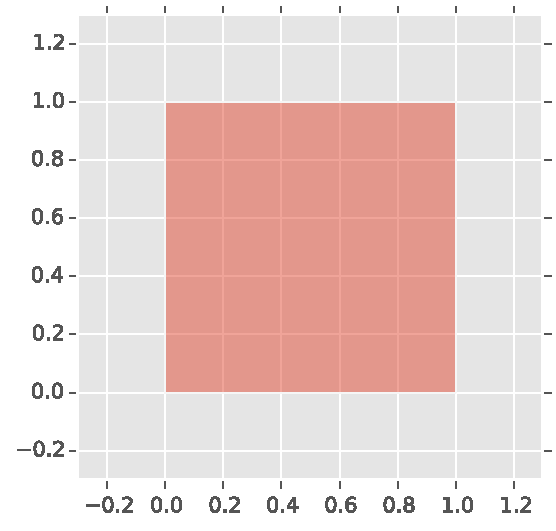
\includegraphics[max size={\textwidth}{\textheight}]{Arnold_cat_map_files/Arnold_cat_map_28_0.pdf}
    \par
    \end{center}
            \end{InvisibleVerbatim}
            
        
    


    % Make sure that atleast 4 lines are below the HR
    \needspace{4\baselineskip}

    
        \vspace{6pt}
        \makebox[0.1\linewidth]{\smaller\hfill\tt\color{nbframe-in-prompt}In\hspace{4pt}{[}25{]}:\hspace{4pt}}\\*
        \vspace{-2.65\baselineskip}
        \begin{ColorVerbatim}
            \vspace{-0.7\baselineskip}
            \begin{Verbatim}[commandchars=\\\{\}]
\PY{c}{\PYZsh{}theta = np.pi / 4.}
\PY{c}{\PYZsh{}R = np.array([np.cos(theta), np.sin(theta), \PYZhy{}np.sin(theta), np.cos(theta)]).reshape((2,2) )}

\PY{c}{\PYZsh{}rotated\PYZus{}square\PYZus{}vertices = [np.dot(R, vertex) for vertex in unit\PYZus{}square.vertices]}
\PY{c}{\PYZsh{}rotated\PYZus{}square = DirectedPolygon(rotated\PYZus{}square\PYZus{}vertices)}

\PY{c}{\PYZsh{}rotated\PYZus{}square.draw()}
\end{Verbatim}

            
                \vspace{-0.2\baselineskip}
            
        \end{ColorVerbatim}
    


    % Make sure that atleast 4 lines are below the HR
    \needspace{4\baselineskip}

    
        \vspace{6pt}
        \makebox[0.1\linewidth]{\smaller\hfill\tt\color{nbframe-in-prompt}In\hspace{4pt}{[}26{]}:\hspace{4pt}}\\*
        \vspace{-2.65\baselineskip}
        \begin{ColorVerbatim}
            \vspace{-0.7\baselineskip}
            \begin{Verbatim}[commandchars=\\\{\}]
\PY{k}{def} \PY{n+nf}{find\PYZus{}starting\PYZus{}point}\PY{p}{(}\PY{n}{polygon1}\PY{p}{,} \PY{n}{polygon2}\PY{p}{)}\PY{p}{:}
    \PY{l+s+sd}{\PYZdq{}\PYZdq{}\PYZdq{}Find the starting point of the intersection of two polygons}
\PY{l+s+sd}{    Returns None if they do not intersect\PYZdq{}\PYZdq{}\PYZdq{}}
    
    \PY{k}{for} \PY{n}{i} \PY{o+ow}{in} \PY{n+nb}{range}\PY{p}{(}\PY{n+nb}{len}\PY{p}{(}\PY{n}{polygon1}\PY{o}{.}\PY{n}{segments}\PY{p}{)}\PY{p}{)}\PY{p}{:}
        \PY{k}{for} \PY{n}{j} \PY{o+ow}{in} \PY{n+nb}{range}\PY{p}{(}\PY{n+nb}{len}\PY{p}{(}\PY{n}{polygon2}\PY{o}{.}\PY{n}{segments}\PY{p}{)}\PY{p}{)}\PY{p}{:}
            
            \PY{n}{segment1} \PY{o}{=} \PY{n}{polygon1}\PY{o}{.}\PY{n}{segments}\PY{p}{[}\PY{n}{i}\PY{p}{]}
            \PY{n}{segment2} \PY{o}{=} \PY{n}{polygon2}\PY{o}{.}\PY{n}{segments}\PY{p}{[}\PY{n}{i}\PY{p}{]}
            
            \PY{n}{intersection} \PY{o}{=} \PY{n}{find\PYZus{}intersection\PYZus{}segments}\PY{p}{(}\PY{n}{segment1}\PY{p}{,} \PY{n}{segment2}\PY{p}{)}
            
            \PY{k}{if} \PY{n}{intersection}\PY{p}{:}
                \PY{k}{return} \PY{p}{(}\PY{n}{intersection}\PY{p}{[}\PY{l+m+mi}{1}\PY{p}{]}\PY{p}{,} \PY{n}{i}\PY{p}{,} \PY{n}{j}\PY{p}{)}  \PY{c}{\PYZsh{} don\PYZsq{}t need the intersection time}
            
    \PY{k}{return} \PY{n+nb+bp}{None}
            
    

\PY{k}{def} \PY{n+nf}{intersection\PYZus{}polygons}\PY{p}{(}\PY{n}{polygon1}\PY{p}{,} \PY{n}{polygon2}\PY{p}{)}\PY{p}{:}
    \PY{l+s+sd}{\PYZdq{}\PYZdq{}\PYZdq{}Calculate intersection of two (convex) polygons}
\PY{l+s+sd}{    First find an intersection point.}
\PY{l+s+sd}{    Then follow this around by taking consecutive pieces of each polygon?}
\PY{l+s+sd}{    \PYZdq{}\PYZdq{}\PYZdq{}}
    
    \PY{n}{starting\PYZus{}point}\PY{p}{,} \PY{n}{i}\PY{p}{,} \PY{n}{j} \PY{o}{=} \PY{n}{find\PYZus{}starting\PYZus{}point}\PY{p}{(}\PY{n}{polygon1}\PY{p}{,} \PY{n}{polygon2}\PY{p}{)}
    \PY{c}{\PYZsh{} i is the number of the segment of the first polygon, j of the second}
    
    \PY{k}{if} \PY{n}{starting\PYZus{}point} \PY{o+ow}{is} \PY{n+nb+bp}{None}\PY{p}{:}
        \PY{k}{return} \PY{n+nb+bp}{None}
    
    \PY{n}{intersection\PYZus{}path} \PY{o}{=} \PY{p}{[}\PY{n}{starting\PYZus{}point}\PY{p}{]}
    
    \PY{n}{current\PYZus{}segment} \PY{o}{=} \PY{n}{polygon2}\PY{o}{.}\PY{n}{segments}\PY{p}{[}\PY{n}{j}\PY{p}{]}
    \PY{n}{remainder} \PY{o}{=} \PY{n}{DirectedLineSegment}\PY{p}{(}\PY{n}{starting\PYZus{}point}\PY{p}{,} \PY{n}{current\PYZus{}segment}\PY{o}{.}\PY{n}{end}\PY{p}{)}
    
\PY{c}{\PYZsh{}    find\PYZus{}intersection\PYZus{}segments(remainder }
\end{Verbatim}

            
                \vspace{-0.2\baselineskip}
            
        \end{ColorVerbatim}
    


    % Make sure that atleast 4 lines are below the HR
    \needspace{4\baselineskip}

    
        \vspace{6pt}
        \makebox[0.1\linewidth]{\smaller\hfill\tt\color{nbframe-in-prompt}In\hspace{4pt}{[}27{]}:\hspace{4pt}}\\*
        \vspace{-2.65\baselineskip}
        \begin{ColorVerbatim}
            \vspace{-0.7\baselineskip}
            \begin{Verbatim}[commandchars=\\\{\}]
\PY{k}{def} \PY{n+nf}{test\PYZus{}find\PYZus{}starting\PYZus{}point}\PY{p}{(}\PY{p}{)}\PY{p}{:}
    
    \PY{n}{unit\PYZus{}square} \PY{o}{=} \PY{n}{DirectedPolygon}\PY{p}{(}\PY{p}{[}\PY{p}{(}\PY{l+m+mf}{0.}\PY{p}{,}\PY{l+m+mf}{0.}\PY{p}{)}\PY{p}{,} \PY{p}{(}\PY{l+m+mf}{1.}\PY{p}{,}\PY{l+m+mf}{0.}\PY{p}{)}\PY{p}{,} \PY{p}{(}\PY{l+m+mf}{1.}\PY{p}{,}\PY{l+m+mf}{1.}\PY{p}{)}\PY{p}{,} \PY{p}{(}\PY{l+m+mf}{0.}\PY{p}{,}\PY{l+m+mf}{1.}\PY{p}{)}\PY{p}{]}\PY{p}{)}
    
    \PY{n}{theta} \PY{o}{=} \PY{n}{np}\PY{o}{.}\PY{n}{pi} \PY{o}{/} \PY{l+m+mf}{4.}
    \PY{n}{R} \PY{o}{=} \PY{n}{np}\PY{o}{.}\PY{n}{array}\PY{p}{(}\PY{p}{[}\PY{n}{np}\PY{o}{.}\PY{n}{cos}\PY{p}{(}\PY{n}{theta}\PY{p}{)}\PY{p}{,} \PY{n}{np}\PY{o}{.}\PY{n}{sin}\PY{p}{(}\PY{n}{theta}\PY{p}{)}\PY{p}{,} \PY{o}{\PYZhy{}}\PY{n}{np}\PY{o}{.}\PY{n}{sin}\PY{p}{(}\PY{n}{theta}\PY{p}{)}\PY{p}{,} \PY{n}{np}\PY{o}{.}\PY{n}{cos}\PY{p}{(}\PY{n}{theta}\PY{p}{)}\PY{p}{]}\PY{p}{)}\PY{o}{.}\PY{n}{reshape}\PY{p}{(}\PY{p}{(}\PY{l+m+mi}{2}\PY{p}{,}\PY{l+m+mi}{2}\PY{p}{)} \PY{p}{)}
    
    \PY{n}{rotated\PYZus{}square\PYZus{}vertices} \PY{o}{=} \PY{p}{[}\PY{n}{np}\PY{o}{.}\PY{n}{dot}\PY{p}{(}\PY{n}{R}\PY{p}{,} \PY{n}{vertex}\PY{p}{)} \PY{k}{for} \PY{n}{vertex} \PY{o+ow}{in} \PY{n}{unit\PYZus{}square}\PY{o}{.}\PY{n}{vertices}\PY{p}{]}
    \PY{n}{rotated\PYZus{}square} \PY{o}{=} \PY{n}{DirectedPolygon}\PY{p}{(}\PY{n}{rotated\PYZus{}square\PYZus{}vertices}\PY{p}{)}
    
    
    \PY{n}{starting\PYZus{}point} \PY{o}{=} \PY{n}{find\PYZus{}starting\PYZus{}point}\PY{p}{(}\PY{n}{unit\PYZus{}square}\PY{p}{,} \PY{n}{rotated\PYZus{}square}\PY{p}{)}
    
    \PY{k}{assert} \PY{n}{starting\PYZus{}point}\PY{p}{[}\PY{l+m+mi}{0}\PY{p}{]} \PY{o}{==} \PY{l+m+mf}{0.0}
    \PY{k}{assert} \PY{n+nb}{all}\PY{p}{(}\PY{n}{starting\PYZus{}point}\PY{p}{[}\PY{l+m+mi}{1}\PY{p}{]} \PY{o}{==} \PY{n}{np}\PY{o}{.}\PY{n}{array}\PY{p}{(}\PY{p}{[}\PY{l+m+mf}{0.0}\PY{p}{,} \PY{l+m+mf}{0.0}\PY{p}{]}\PY{p}{)}\PY{p}{)}
    
    
    \PY{n}{new\PYZus{}square} \PY{o}{=} \PY{p}{[}\PY{n}{vertex} \PY{o}{+} \PY{n}{np}\PY{o}{.}\PY{n}{array}\PY{p}{(}\PY{p}{[}\PY{l+m+mf}{10.}\PY{p}{,} \PY{l+m+mf}{0.}\PY{p}{]}\PY{p}{)} \PY{k}{for} \PY{n}{vertex} \PY{o+ow}{in} \PY{n}{unit\PYZus{}square}\PY{o}{.}\PY{n}{vertices}\PY{p}{]}
    
    \PY{n}{starting\PYZus{}point} \PY{o}{=} \PY{n}{find\PYZus{}starting\PYZus{}point}\PY{p}{(}\PY{n}{unit\PYZus{}square}\PY{p}{,} \PY{n}{new\PYZus{}square}\PY{p}{)}
    
    \PY{k}{assert} \PY{n}{starting\PYZus{}point} \PY{o}{==} \PY{n+nb+bp}{None}
\end{Verbatim}

            
                \vspace{-0.2\baselineskip}
            
        \end{ColorVerbatim}
    


    % Make sure that atleast 4 lines are below the HR
    \needspace{4\baselineskip}

    
        \vspace{6pt}
        \makebox[0.1\linewidth]{\smaller\hfill\tt\color{nbframe-in-prompt}In\hspace{4pt}{[}28{]}:\hspace{4pt}}\\*
        \vspace{-2.65\baselineskip}
        \begin{ColorVerbatim}
            \vspace{-0.7\baselineskip}
            \begin{Verbatim}[commandchars=\\\{\}]
\PY{n}{new\PYZus{}square\PYZus{}vertices} \PY{o}{=} \PY{p}{[}\PY{n}{vertex} \PY{o}{+} \PY{n}{np}\PY{o}{.}\PY{n}{array}\PY{p}{(}\PY{p}{[}\PY{l+m+mf}{10.}\PY{p}{,} \PY{l+m+mf}{0.}\PY{p}{]}\PY{p}{)} \PY{k}{for} \PY{n}{vertex} \PY{o+ow}{in} \PY{n}{unit\PYZus{}square}\PY{o}{.}\PY{n}{vertices}\PY{p}{]}
\PY{n}{new\PYZus{}square} \PY{o}{=} \PY{n}{DirectedPolygon}\PY{p}{(}\PY{n}{new\PYZus{}square\PYZus{}vertices}\PY{p}{)}
\PY{n}{find\PYZus{}starting\PYZus{}point}\PY{p}{(}\PY{n}{unit\PYZus{}square}\PY{p}{,} \PY{n}{new\PYZus{}square}\PY{p}{)}
\end{Verbatim}

            
                \vspace{-0.2\baselineskip}
            
        \end{ColorVerbatim}
    


    % Make sure that atleast 4 lines are below the HR
    \needspace{4\baselineskip}

    
        \vspace{6pt}
        \makebox[0.1\linewidth]{\smaller\hfill\tt\color{nbframe-in-prompt}In\hspace{4pt}{[}29{]}:\hspace{4pt}}\\*
        \vspace{-2.65\baselineskip}
        \begin{ColorVerbatim}
            \vspace{-0.7\baselineskip}
            \begin{Verbatim}[commandchars=\\\{\}]
\PY{n}{new\PYZus{}square}
\end{Verbatim}

            
                \vspace{-0.2\baselineskip}
            
        \end{ColorVerbatim}
    

    

        % If the first block is an image, minipage the image.  Else
        % request a certain amount of space for the input text.
        \needspace{4\baselineskip}
        
        

            % Add document contents.
            
                \makebox[0.1\linewidth]{\smaller\hfill\tt\color{nbframe-out-prompt}Out\hspace{4pt}{[}29{]}:\hspace{4pt}}\\*
                \vspace{-2.55\baselineskip}\begin{InvisibleVerbatim}
                \vspace{-0.5\baselineskip}
    \begin{alltt}[DirectedLineSegment([10, 0], [11, 0]), DirectedLineSegment([11, 0],
[11, 1]), DirectedLineSegment([11, 1], [10, 1]),
DirectedLineSegment([10, 1], [10, 0])]\end{alltt}

            \end{InvisibleVerbatim}
            
        
    


    % Make sure that atleast 4 lines are below the HR
    \needspace{4\baselineskip}

    
        \vspace{6pt}
        \makebox[0.1\linewidth]{\smaller\hfill\tt\color{nbframe-in-prompt}In\hspace{4pt}{[}30{]}:\hspace{4pt}}\\*
        \vspace{-2.65\baselineskip}
        \begin{ColorVerbatim}
            \vspace{-0.7\baselineskip}
            \begin{Verbatim}[commandchars=\\\{\}]
\PY{n}{unit\PYZus{}square}
\end{Verbatim}

            
                \vspace{-0.2\baselineskip}
            
        \end{ColorVerbatim}
    

    

        % If the first block is an image, minipage the image.  Else
        % request a certain amount of space for the input text.
        \needspace{4\baselineskip}
        
        

            % Add document contents.
            
                \makebox[0.1\linewidth]{\smaller\hfill\tt\color{nbframe-out-prompt}Out\hspace{4pt}{[}30{]}:\hspace{4pt}}\\*
                \vspace{-2.55\baselineskip}\begin{InvisibleVerbatim}
                \vspace{-0.5\baselineskip}
    \begin{alltt}[DirectedLineSegment([0, 0], [1, 0]), DirectedLineSegment([1, 0], [1,
1]), DirectedLineSegment([1, 1], [0, 1]), DirectedLineSegment([0, 1],
[0, 0])]\end{alltt}

            \end{InvisibleVerbatim}
            
        
    
\section{Mapping vertices and polygons}A \emph{map} is a function $f : \mathbb{R}^2 \to \mathbb{R}^2.$ Our
first example is the map
$\mathbf{x} \overset{f}{\mapsto} \mathsf{M} \cdot \mathbf{x}$, where

\[\mathsf{M} := \begin{pmatrix} 2 & 1 \\ 1 & 1 \end{pmatrix}:\]

    % Make sure that atleast 4 lines are below the HR
    \needspace{4\baselineskip}

    
        \vspace{6pt}
        \makebox[0.1\linewidth]{\smaller\hfill\tt\color{nbframe-in-prompt}In\hspace{4pt}{[}31{]}:\hspace{4pt}}\\*
        \vspace{-2.65\baselineskip}
        \begin{ColorVerbatim}
            \vspace{-0.7\baselineskip}
            \begin{Verbatim}[commandchars=\\\{\}]
\PY{n}{M} \PY{o}{=} \PY{n}{np}\PY{o}{.}\PY{n}{array}\PY{p}{(}\PY{p}{[}\PY{p}{[}\PY{l+m+mi}{2}\PY{p}{,} \PY{l+m+mi}{1}\PY{p}{]}\PY{p}{,} \PY{p}{[}\PY{l+m+mi}{1}\PY{p}{,} \PY{l+m+mi}{1}\PY{p}{]}\PY{p}{]}\PY{p}{)}
\PY{k}{print} \PY{n}{M}
\end{Verbatim}

            
                \vspace{-0.2\baselineskip}
            
        \end{ColorVerbatim}
    

    

        % If the first block is an image, minipage the image.  Else
        % request a certain amount of space for the input text.
        \needspace{4\baselineskip}
        
        

            % Add document contents.
            
                \begin{InvisibleVerbatim}
                \vspace{-0.5\baselineskip}
    \begin{alltt}[[2 1]
 [1 1]]
\end{alltt}

            \end{InvisibleVerbatim}
            
        
    


    % Make sure that atleast 4 lines are below the HR
    \needspace{4\baselineskip}

    
        \vspace{6pt}
        \makebox[0.1\linewidth]{\smaller\hfill\tt\color{nbframe-in-prompt}In\hspace{4pt}{[}32{]}:\hspace{4pt}}\\*
        \vspace{-2.65\baselineskip}
        \begin{ColorVerbatim}
            \vspace{-0.7\baselineskip}
            \begin{Verbatim}[commandchars=\\\{\}]
\PY{k}{def} \PY{n+nf}{f}\PY{p}{(}\PY{n}{x}\PY{p}{)}\PY{p}{:}
    \PY{k}{return} \PY{n}{np}\PY{o}{.}\PY{n}{dot}\PY{p}{(}\PY{n}{M}\PY{p}{,} \PY{n}{x}\PY{p}{)}
\end{Verbatim}

            
                \vspace{-0.2\baselineskip}
            
        \end{ColorVerbatim}
    
\texttt{f} applies the map to a single vertex. Now we need something to
apply it to all the vertices of a polygon, creating a new polygon:

    % Make sure that atleast 4 lines are below the HR
    \needspace{4\baselineskip}

    
        \vspace{6pt}
        \makebox[0.1\linewidth]{\smaller\hfill\tt\color{nbframe-in-prompt}In\hspace{4pt}{[}33{]}:\hspace{4pt}}\\*
        \vspace{-2.65\baselineskip}
        \begin{ColorVerbatim}
            \vspace{-0.7\baselineskip}
            \begin{Verbatim}[commandchars=\\\{\}]
\PY{k}{def} \PY{n+nf}{map\PYZus{}poly}\PY{p}{(}\PY{n}{f}\PY{p}{,} \PY{n}{poly}\PY{p}{)}\PY{p}{:}
    \PY{l+s+sd}{\PYZdq{}\PYZdq{}\PYZdq{}Apply the map f to each vertex of the Poygon poly, returning a new Polygon\PYZdq{}\PYZdq{}\PYZdq{}}
    
    \PY{n}{vertices} \PY{o}{=} \PY{n}{poly}\PY{o}{.}\PY{n}{vertices}
    \PY{n}{new\PYZus{}vertices} \PY{o}{=} \PY{p}{[}\PY{n}{f}\PY{p}{(}\PY{n}{vertex}\PY{p}{)} \PY{k}{for} \PY{n}{vertex} \PY{o+ow}{in} \PY{n}{vertices}\PY{p}{]}
    
    \PY{k}{return} \PY{n}{DirectedPolygon}\PY{p}{(}\PY{n}{new\PYZus{}vertices}\PY{p}{)}
\end{Verbatim}

            
                \vspace{-0.2\baselineskip}
            
        \end{ColorVerbatim}
    
Let's apply our map \texttt{f} to the unit square, and then apply it
again to get the second iterate $f^{(2)} := f \circ f$:

    % Make sure that atleast 4 lines are below the HR
    \needspace{4\baselineskip}

    
        \vspace{6pt}
        \makebox[0.1\linewidth]{\smaller\hfill\tt\color{nbframe-in-prompt}In\hspace{4pt}{[}34{]}:\hspace{4pt}}\\*
        \vspace{-2.65\baselineskip}
        \begin{ColorVerbatim}
            \vspace{-0.7\baselineskip}
            \begin{Verbatim}[commandchars=\\\{\}]
\PY{n}{unit\PYZus{}square} \PY{o}{=} \PY{n}{DirectedPolygon}\PY{p}{(}\PY{p}{[}\PY{p}{(}\PY{l+m+mf}{0.}\PY{p}{,}\PY{l+m+mf}{0.}\PY{p}{)}\PY{p}{,} \PY{p}{(}\PY{l+m+mf}{1.}\PY{p}{,}\PY{l+m+mf}{0.}\PY{p}{)}\PY{p}{,} \PY{p}{(}\PY{l+m+mf}{1.}\PY{p}{,}\PY{l+m+mf}{1.}\PY{p}{)}\PY{p}{,} \PY{p}{(}\PY{l+m+mf}{0.}\PY{p}{,}\PY{l+m+mf}{1.}\PY{p}{)}\PY{p}{]}\PY{p}{)}

\PY{n}{iterates} \PY{o}{=} \PY{p}{[}\PY{n}{unit\PYZus{}square}\PY{p}{]}
\PY{n}{iterates}\PY{o}{.}\PY{n}{append}\PY{p}{(}\PY{n}{map\PYZus{}poly}\PY{p}{(}\PY{n}{f}\PY{p}{,} \PY{n}{iterates}\PY{p}{[}\PY{o}{\PYZhy{}}\PY{l+m+mi}{1}\PY{p}{]}\PY{p}{)}\PY{p}{)}
\end{Verbatim}

            
                \vspace{-0.2\baselineskip}
            
        \end{ColorVerbatim}
    
Let us draw the original unit square and its first iterate:

    % Make sure that atleast 4 lines are below the HR
    \needspace{4\baselineskip}

    
        \vspace{6pt}
        \makebox[0.1\linewidth]{\smaller\hfill\tt\color{nbframe-in-prompt}In\hspace{4pt}{[}35{]}:\hspace{4pt}}\\*
        \vspace{-2.65\baselineskip}
        \begin{ColorVerbatim}
            \vspace{-0.7\baselineskip}
            \begin{Verbatim}[commandchars=\\\{\}]
\PY{k}{for} \PY{n}{i} \PY{o+ow}{in} \PY{n}{iterates}\PY{p}{[}\PY{l+m+mi}{0}\PY{p}{:}\PY{l+m+mi}{2}\PY{p}{]}\PY{p}{:}
    \PY{n}{i}\PY{o}{.}\PY{n}{draw}\PY{p}{(}\PY{p}{)}

\PY{n}{plt}\PY{o}{.}\PY{n}{grid}\PY{p}{(}\PY{p}{)}

\PY{n}{plt}\PY{o}{.}\PY{n}{axis}\PY{p}{(}\PY{l+s}{\PYZsq{}}\PY{l+s}{scaled}\PY{l+s}{\PYZsq{}}\PY{p}{)}

\PY{n}{plt}\PY{o}{.}\PY{n}{show}\PY{p}{(}\PY{p}{)}
\end{Verbatim}

            
                \vspace{-0.2\baselineskip}
            
        \end{ColorVerbatim}
    

    

        % If the first block is an image, minipage the image.  Else
        % request a certain amount of space for the input text.
        \needspace{4\baselineskip}
        
        

            % Add document contents.
            
                \begin{InvisibleVerbatim}
                \vspace{-0.5\baselineskip}\begin{center}
    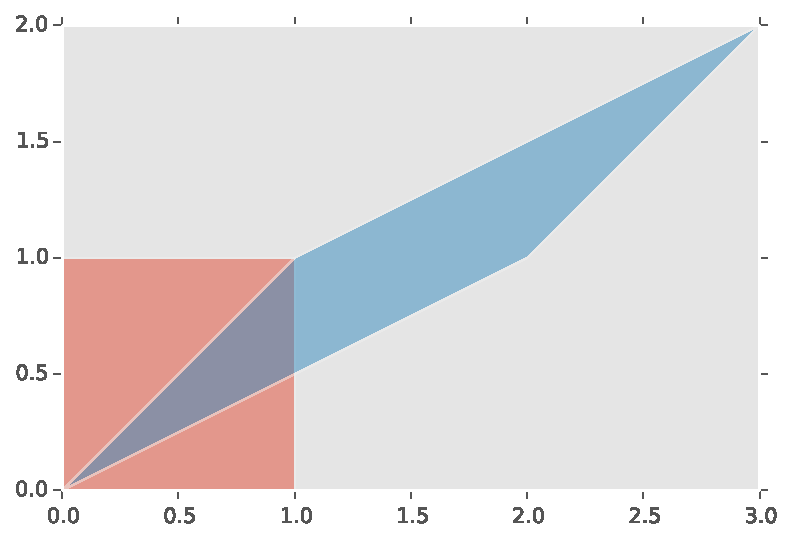
\includegraphics[max size={\textwidth}{\textheight}]{Arnold_cat_map_files/Arnold_cat_map_44_0.pdf}
    \par
    \end{center}
            \end{InvisibleVerbatim}
            
        
    


    % Make sure that atleast 4 lines are below the HR
    \needspace{4\baselineskip}

    
        \vspace{6pt}
        \makebox[0.1\linewidth]{\smaller\hfill\tt\color{nbframe-in-prompt}In\hspace{4pt}{[}36{]}:\hspace{4pt}}\\*
        \vspace{-2.65\baselineskip}
        \begin{ColorVerbatim}
            \vspace{-0.7\baselineskip}
            \begin{Verbatim}[commandchars=\\\{\}]
\PY{k}{def} \PY{n+nf}{draw\PYZus{}iterates}\PY{p}{(}\PY{n}{n}\PY{p}{)}\PY{p}{:}
    \PY{l+s+sd}{\PYZdq{}\PYZdq{}\PYZdq{}Draw iterates up to and including the nth\PYZdq{}\PYZdq{}\PYZdq{}}
    
    \PY{k}{while} \PY{n+nb}{len}\PY{p}{(}\PY{n}{iterates}\PY{p}{)} \PY{o}{\PYZlt{}} \PY{n}{n}\PY{o}{+}\PY{l+m+mi}{1}\PY{p}{:}
        \PY{n}{iterates}\PY{o}{.}\PY{n}{append}\PY{p}{(}\PY{n}{map\PYZus{}poly}\PY{p}{(}\PY{n}{f}\PY{p}{,} \PY{n}{iterates}\PY{p}{[}\PY{o}{\PYZhy{}}\PY{l+m+mi}{1}\PY{p}{]}\PY{p}{)}\PY{p}{)}
    
    \PY{k}{for} \PY{n}{i} \PY{o+ow}{in} \PY{n}{iterates}\PY{p}{[}\PY{l+m+mi}{0}\PY{p}{:}\PY{n}{n}\PY{o}{+}\PY{l+m+mi}{1}\PY{p}{]}\PY{p}{:}
        \PY{n}{i}\PY{o}{.}\PY{n}{draw}\PY{p}{(}\PY{p}{)}
    
    \PY{n}{plt}\PY{o}{.}\PY{n}{grid}\PY{p}{(}\PY{p}{)}
    
    \PY{n}{plt}\PY{o}{.}\PY{n}{axis}\PY{p}{(}\PY{l+s}{\PYZsq{}}\PY{l+s}{scaled}\PY{l+s}{\PYZsq{}}\PY{p}{)}
    
    \PY{n}{plt}\PY{o}{.}\PY{n}{show}\PY{p}{(}\PY{p}{)}
\end{Verbatim}

            
                \vspace{-0.2\baselineskip}
            
        \end{ColorVerbatim}
    
Let's make a function to draw higher iterates:We can add the second iterate to the mix:

    % Make sure that atleast 4 lines are below the HR
    \needspace{4\baselineskip}

    
        \vspace{6pt}
        \makebox[0.1\linewidth]{\smaller\hfill\tt\color{nbframe-in-prompt}In\hspace{4pt}{[}37{]}:\hspace{4pt}}\\*
        \vspace{-2.65\baselineskip}
        \begin{ColorVerbatim}
            \vspace{-0.7\baselineskip}
            \begin{Verbatim}[commandchars=\\\{\}]
\PY{n}{draw\PYZus{}iterates}\PY{p}{(}\PY{l+m+mi}{2}\PY{p}{)}
\end{Verbatim}

            
                \vspace{-0.2\baselineskip}
            
        \end{ColorVerbatim}
    

    

        % If the first block is an image, minipage the image.  Else
        % request a certain amount of space for the input text.
        \needspace{4\baselineskip}
        
        

            % Add document contents.
            
                \begin{InvisibleVerbatim}
                \vspace{-0.5\baselineskip}\begin{center}
    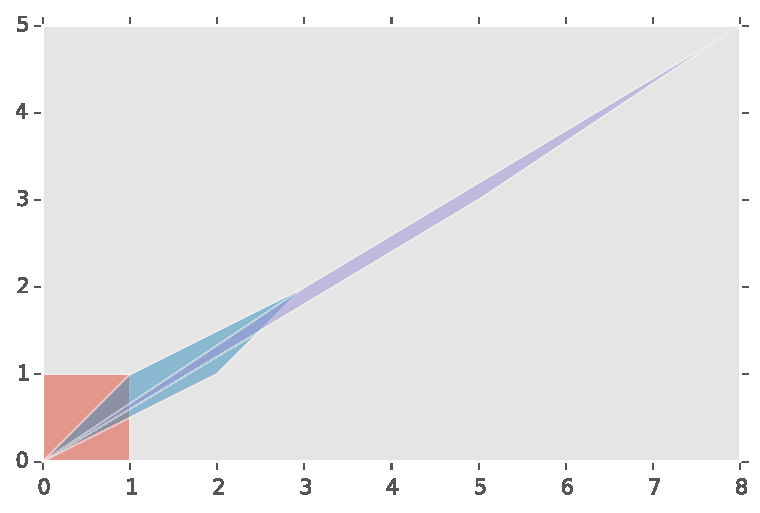
\includegraphics[max size={\textwidth}{\textheight}]{Arnold_cat_map_files/Arnold_cat_map_48_0.pdf}
    \par
    \end{center}
            \end{InvisibleVerbatim}
            
        
    
And why not add the next as well, just for fun:

    % Make sure that atleast 4 lines are below the HR
    \needspace{4\baselineskip}

    
        \vspace{6pt}
        \makebox[0.1\linewidth]{\smaller\hfill\tt\color{nbframe-in-prompt}In\hspace{4pt}{[}38{]}:\hspace{4pt}}\\*
        \vspace{-2.65\baselineskip}
        \begin{ColorVerbatim}
            \vspace{-0.7\baselineskip}
            \begin{Verbatim}[commandchars=\\\{\}]
\PY{n}{draw\PYZus{}iterates}\PY{p}{(}\PY{l+m+mi}{3}\PY{p}{)}
\end{Verbatim}

            
                \vspace{-0.2\baselineskip}
            
        \end{ColorVerbatim}
    

    

        % If the first block is an image, minipage the image.  Else
        % request a certain amount of space for the input text.
        \needspace{4\baselineskip}
        
        

            % Add document contents.
            
                \begin{InvisibleVerbatim}
                \vspace{-0.5\baselineskip}\begin{center}
    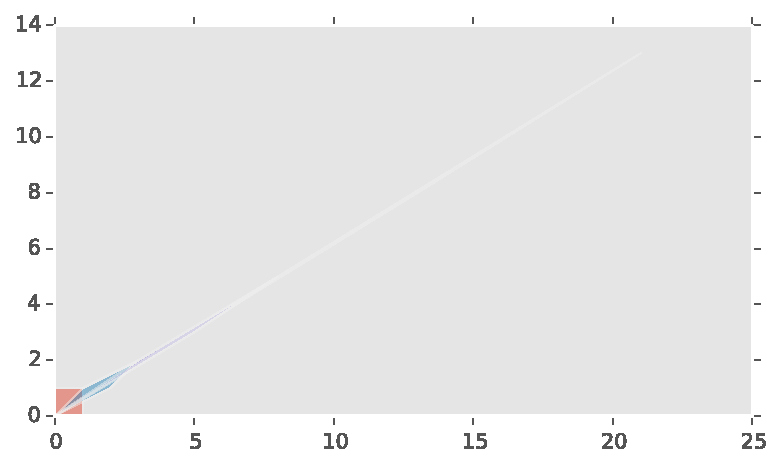
\includegraphics[max size={\textwidth}{\textheight}]{Arnold_cat_map_files/Arnold_cat_map_50_0.pdf}
    \par
    \end{center}
            \end{InvisibleVerbatim}
            
        
    
It is clear that the resulting parallelogram is aligning itself along a
line. This line is the \emph{unstable manifold} of the origin. Since the
map is \emph{linear}, the unstable manifold is equal to the unstable
\emph{subspace} of the linearization (which is just the map itself,
since it is linear).

The unstable subspace is given by the eigenvector whose eigenvalue is
larger than $1$. Let's calculate these:

    % Make sure that atleast 4 lines are below the HR
    \needspace{4\baselineskip}

    
        \vspace{6pt}
        \makebox[0.1\linewidth]{\smaller\hfill\tt\color{nbframe-in-prompt}In\hspace{4pt}{[}39{]}:\hspace{4pt}}\\*
        \vspace{-2.65\baselineskip}
        \begin{ColorVerbatim}
            \vspace{-0.7\baselineskip}
            \begin{Verbatim}[commandchars=\\\{\}]
\PY{k+kn}{from} \PY{n+nn}{numpy} \PY{k+kn}{import} \PY{n}{linalg}
\end{Verbatim}

            
                \vspace{-0.2\baselineskip}
            
        \end{ColorVerbatim}
    


    % Make sure that atleast 4 lines are below the HR
    \needspace{4\baselineskip}

    
        \vspace{6pt}
        \makebox[0.1\linewidth]{\smaller\hfill\tt\color{nbframe-in-prompt}In\hspace{4pt}{[}40{]}:\hspace{4pt}}\\*
        \vspace{-2.65\baselineskip}
        \begin{ColorVerbatim}
            \vspace{-0.7\baselineskip}
            \begin{Verbatim}[commandchars=\\\{\}]
\PY{n}{lamb}\PY{p}{,} \PY{n}{v} \PY{o}{=} \PY{n}{linalg}\PY{o}{.}\PY{n}{eig}\PY{p}{(}\PY{n}{M}\PY{p}{)}
\PY{n}{lamb}\PY{p}{,} \PY{n}{v}
\end{Verbatim}

            
                \vspace{-0.2\baselineskip}
            
        \end{ColorVerbatim}
    

    

        % If the first block is an image, minipage the image.  Else
        % request a certain amount of space for the input text.
        \needspace{4\baselineskip}
        
        

            % Add document contents.
            
                \makebox[0.1\linewidth]{\smaller\hfill\tt\color{nbframe-out-prompt}Out\hspace{4pt}{[}40{]}:\hspace{4pt}}\\*
                \vspace{-2.55\baselineskip}\begin{InvisibleVerbatim}
                \vspace{-0.5\baselineskip}
    \begin{alltt}(array([ 2.61803399,  0.38196601]),
 array([[ 0.85065081, -0.52573111],
       [ 0.52573111,  0.85065081]]))\end{alltt}

            \end{InvisibleVerbatim}
            
        
    
Note that the eigenvectores are returned in the \emph{columns} of the
matrix. We can now add the eigenvector to our plot:

    % Make sure that atleast 4 lines are below the HR
    \needspace{4\baselineskip}

    
        \vspace{6pt}
        \makebox[0.1\linewidth]{\smaller\hfill\tt\color{nbframe-in-prompt}In\hspace{4pt}{[}41{]}:\hspace{4pt}}\\*
        \vspace{-2.65\baselineskip}
        \begin{ColorVerbatim}
            \vspace{-0.7\baselineskip}
            \begin{Verbatim}[commandchars=\\\{\}]
\PY{n}{fig}\PY{p}{,} \PY{p}{(}\PY{n}{ax1}\PY{p}{)} \PY{o}{=} \PY{n}{plt}\PY{o}{.}\PY{n}{subplots}\PY{p}{(}\PY{p}{)}

\PY{n}{plt}\PY{o}{.}\PY{n}{plot}\PY{p}{(}\PY{p}{[}\PY{l+m+mi}{0}\PY{p}{,} \PY{n}{v}\PY{p}{[}\PY{l+m+mi}{0}\PY{p}{,}\PY{l+m+mi}{0}\PY{p}{]}\PY{o}{*}\PY{l+m+mi}{8}\PY{p}{]}\PY{p}{,} \PY{p}{[}\PY{l+m+mi}{0}\PY{p}{,} \PY{n}{v}\PY{p}{[}\PY{l+m+mi}{1}\PY{p}{,}\PY{l+m+mi}{0}\PY{p}{]}\PY{o}{*}\PY{l+m+mi}{8}\PY{p}{]}\PY{p}{,} \PY{l+s}{\PYZsq{}}\PY{l+s}{k\PYZhy{}\PYZhy{}}\PY{l+s}{\PYZsq{}}\PY{p}{,} \PY{n}{lw}\PY{o}{=}\PY{l+m+mf}{0.5}\PY{p}{)}
\PY{n}{plt}\PY{o}{.}\PY{n}{arrow}\PY{p}{(}\PY{l+m+mi}{0}\PY{p}{,} \PY{l+m+mi}{0}\PY{p}{,} \PY{n}{v}\PY{p}{[}\PY{l+m+mi}{0}\PY{p}{,}\PY{l+m+mi}{0}\PY{p}{]}\PY{o}{*}\PY{l+m+mi}{6}\PY{p}{,} \PY{n}{v}\PY{p}{[}\PY{l+m+mi}{1}\PY{p}{,} \PY{l+m+mi}{0}\PY{p}{]}\PY{o}{*}\PY{l+m+mi}{6}\PY{p}{,} \PY{n}{axes}\PY{o}{=}\PY{n}{ax1}\PY{p}{,} \PY{n}{head\PYZus{}width}\PY{o}{=}\PY{l+m+mf}{0.2}\PY{p}{,} \PY{n}{head\PYZus{}length}\PY{o}{=}\PY{l+m+mf}{0.1}\PY{p}{,} \PY{n}{fc}\PY{o}{=}\PY{l+s}{\PYZdq{}}\PY{l+s}{g}\PY{l+s}{\PYZdq{}}\PY{p}{,} \PY{n}{ec}\PY{o}{=}\PY{l+s}{\PYZdq{}}\PY{l+s}{w}\PY{l+s}{\PYZdq{}}\PY{p}{,} \PY{n}{width}\PY{o}{=}\PY{l+m+mf}{0.05}\PY{p}{)}

\PY{n}{draw\PYZus{}iterates}\PY{p}{(}\PY{l+m+mi}{2}\PY{p}{)}
\end{Verbatim}

            
                \vspace{-0.2\baselineskip}
            
        \end{ColorVerbatim}
    

    

        % If the first block is an image, minipage the image.  Else
        % request a certain amount of space for the input text.
        \needspace{4\baselineskip}
        
        

            % Add document contents.
            
                \begin{InvisibleVerbatim}
                \vspace{-0.5\baselineskip}\begin{center}
    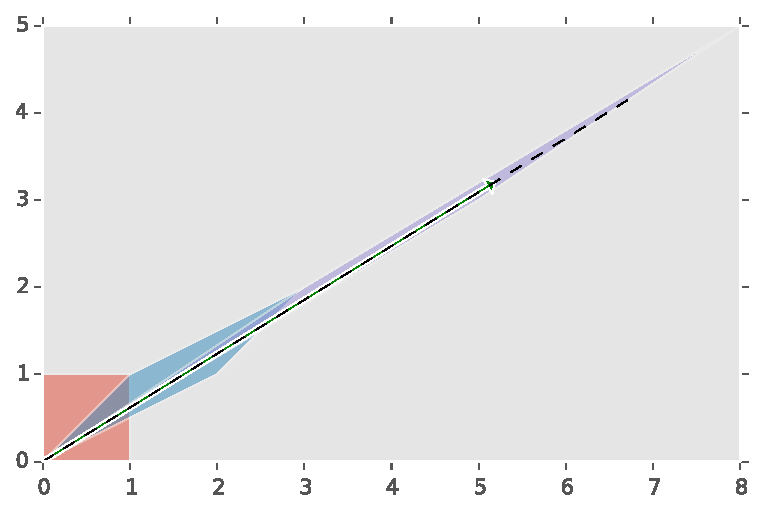
\includegraphics[max size={\textwidth}{\textheight}]{Arnold_cat_map_files/Arnold_cat_map_55_0.pdf}
    \par
    \end{center}
            \end{InvisibleVerbatim}
            
        
    


    % Make sure that atleast 4 lines are below the HR
    \needspace{4\baselineskip}

    
        \vspace{6pt}
        \makebox[0.1\linewidth]{\smaller\hfill\tt\color{nbframe-in-prompt}In\hspace{4pt}{[}42{]}:\hspace{4pt}}\\*
        \vspace{-2.65\baselineskip}
        \begin{ColorVerbatim}
            \vspace{-0.7\baselineskip}
            \begin{Verbatim}[commandchars=\\\{\}]
\PY{n}{plt}\PY{o}{.}\PY{n}{plot}\PY{p}{(}\PY{p}{[}\PY{l+m+mi}{0}\PY{p}{,} \PY{n}{v}\PY{p}{[}\PY{l+m+mi}{0}\PY{p}{,}\PY{l+m+mi}{0}\PY{p}{]}\PY{o}{*}\PY{l+m+mi}{15}\PY{p}{]}\PY{p}{,} \PY{p}{[}\PY{l+m+mi}{0}\PY{p}{,} \PY{n}{v}\PY{p}{[}\PY{l+m+mi}{1}\PY{p}{,}\PY{l+m+mi}{0}\PY{p}{]}\PY{o}{*}\PY{l+m+mi}{15}\PY{p}{]}\PY{p}{,} \PY{l+s}{\PYZsq{}}\PY{l+s}{k\PYZhy{}\PYZhy{}}\PY{l+s}{\PYZsq{}}\PY{p}{,} \PY{n}{lw}\PY{o}{=}\PY{l+m+mf}{0.5}\PY{p}{)}
\PY{n}{plt}\PY{o}{.}\PY{n}{arrow}\PY{p}{(}\PY{l+m+mi}{0}\PY{p}{,} \PY{l+m+mi}{0}\PY{p}{,} \PY{n}{v}\PY{p}{[}\PY{l+m+mi}{0}\PY{p}{,}\PY{l+m+mi}{0}\PY{p}{]}\PY{o}{*}\PY{l+m+mi}{20}\PY{p}{,} \PY{n}{v}\PY{p}{[}\PY{l+m+mi}{1}\PY{p}{,} \PY{l+m+mi}{0}\PY{p}{]}\PY{o}{*}\PY{l+m+mi}{20}\PY{p}{,} \PY{n}{axes}\PY{o}{=}\PY{n}{ax1}\PY{p}{,} \PY{n}{head\PYZus{}width}\PY{o}{=}\PY{l+m+mf}{0.2}\PY{p}{,} \PY{n}{head\PYZus{}length}\PY{o}{=}\PY{l+m+mf}{0.1}\PY{p}{,} \PY{n}{fc}\PY{o}{=}\PY{l+s}{\PYZdq{}}\PY{l+s}{g}\PY{l+s}{\PYZdq{}}\PY{p}{,} \PY{n}{ec}\PY{o}{=}\PY{l+s}{\PYZdq{}}\PY{l+s}{w}\PY{l+s}{\PYZdq{}}\PY{p}{,} \PY{n}{width}\PY{o}{=}\PY{l+m+mf}{0.05}\PY{p}{)}

\PY{n}{draw\PYZus{}iterates}\PY{p}{(}\PY{l+m+mi}{3}\PY{p}{)}
\end{Verbatim}

            
                \vspace{-0.2\baselineskip}
            
        \end{ColorVerbatim}
    

    

        % If the first block is an image, minipage the image.  Else
        % request a certain amount of space for the input text.
        \needspace{4\baselineskip}
        
        

            % Add document contents.
            
                \begin{InvisibleVerbatim}
                \vspace{-0.5\baselineskip}\begin{center}
    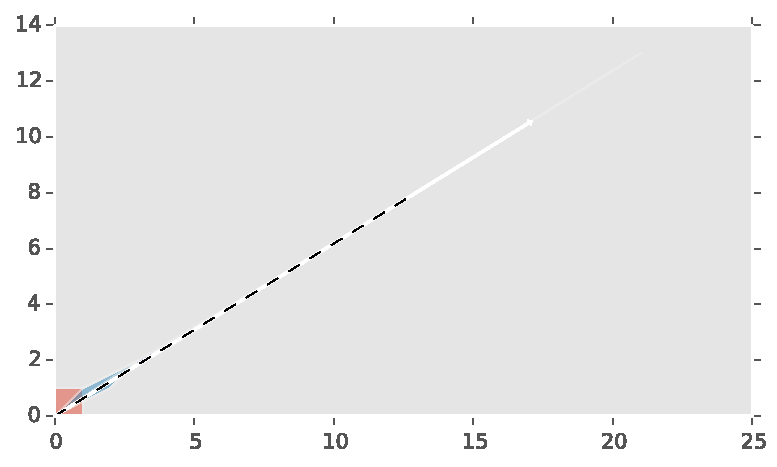
\includegraphics[max size={\textwidth}{\textheight}]{Arnold_cat_map_files/Arnold_cat_map_56_0.pdf}
    \par
    \end{center}
            \end{InvisibleVerbatim}
            
        
    


    % Make sure that atleast 4 lines are below the HR
    \needspace{4\baselineskip}

    
        \vspace{6pt}
        \makebox[0.1\linewidth]{\smaller\hfill\tt\color{nbframe-in-prompt}In\hspace{4pt}{[}43{]}:\hspace{4pt}}\\*
        \vspace{-2.65\baselineskip}
        \begin{ColorVerbatim}
            \vspace{-0.7\baselineskip}
            \begin{Verbatim}[commandchars=\\\{\}]
\PY{n}{ax}\PY{o}{.}
\end{Verbatim}

            
                \vspace{-0.2\baselineskip}
            
        \end{ColorVerbatim}
    

    

        % If the first block is an image, minipage the image.  Else
        % request a certain amount of space for the input text.
        \needspace{4\baselineskip}
        
        

            % Add document contents.
            
                
            \begin{alltt}
          File "<ipython-input-43-8245e8db10a3>", line 1
        ax.
           ^
    SyntaxError: invalid syntax

\end{alltt}
        
            
        
    
\subsection{Interpolating the Arnold cat map}To visualise a bit better the stretching action of the map, we could
think about interpolating between the identity and the cat map. To look
at that, we would like to do some symbolic computations, so we import
the \texttt{sympy} package:

    % Make sure that atleast 4 lines are below the HR
    \needspace{4\baselineskip}

    
        \vspace{6pt}
        \makebox[0.1\linewidth]{\smaller\hfill\tt\color{nbframe-in-prompt}In\hspace{4pt}{[}{]}:\hspace{4pt}}\\*
        \vspace{-2.65\baselineskip}
        \begin{ColorVerbatim}
            \vspace{-0.7\baselineskip}
            \begin{Verbatim}[commandchars=\\\{\}]
\PY{k+kn}{import} \PY{n+nn}{sympy}
\end{Verbatim}

            
                \vspace{-0.2\baselineskip}
            
        \end{ColorVerbatim}
    


    % Make sure that atleast 4 lines are below the HR
    \needspace{4\baselineskip}

    
        \vspace{6pt}
        \makebox[0.1\linewidth]{\smaller\hfill\tt\color{nbframe-in-prompt}In\hspace{4pt}{[}{]}:\hspace{4pt}}\\*
        \vspace{-2.65\baselineskip}
        \begin{ColorVerbatim}
            \vspace{-0.7\baselineskip}
            \begin{Verbatim}[commandchars=\\\{\}]
\PY{k+kn}{from} \PY{n+nn}{sympy} \PY{k+kn}{import} \PY{n}{init\PYZus{}printing}
\PY{n}{init\PYZus{}printing}\PY{p}{(}\PY{p}{)}  \PY{c}{\PYZsh{} turn on pretty printing in the notebook}
\end{Verbatim}

            
                \vspace{-0.2\baselineskip}
            
        \end{ColorVerbatim}
    
Let's define the cat map and the identity matrix:

    % Make sure that atleast 4 lines are below the HR
    \needspace{4\baselineskip}

    
        \vspace{6pt}
        \makebox[0.1\linewidth]{\smaller\hfill\tt\color{nbframe-in-prompt}In\hspace{4pt}{[}{]}:\hspace{4pt}}\\*
        \vspace{-2.65\baselineskip}
        \begin{ColorVerbatim}
            \vspace{-0.7\baselineskip}
            \begin{Verbatim}[commandchars=\\\{\}]
\PY{n}{Identity} \PY{o}{=} \PY{n}{sympy}\PY{o}{.}\PY{n}{Matrix}\PY{p}{(}\PY{p}{[}\PY{p}{[}\PY{l+m+mi}{1}\PY{p}{,} \PY{l+m+mi}{0}\PY{p}{]}\PY{p}{,} \PY{p}{[}\PY{l+m+mi}{0}\PY{p}{,} \PY{l+m+mi}{1}\PY{p}{]}\PY{p}{]}\PY{p}{)}
\PY{n}{CatMap} \PY{o}{=} \PY{n}{sympy}\PY{o}{.}\PY{n}{Matrix}\PY{p}{(}\PY{p}{[}\PY{p}{[}\PY{l+m+mi}{2}\PY{p}{,} \PY{l+m+mi}{1}\PY{p}{]}\PY{p}{,} \PY{p}{[}\PY{l+m+mi}{1}\PY{p}{,} \PY{l+m+mi}{1}\PY{p}{]}\PY{p}{]}\PY{p}{)}

\PY{n}{Identity}\PY{p}{,} \PY{n}{CatMap}
\end{Verbatim}

            
                \vspace{-0.2\baselineskip}
            
        \end{ColorVerbatim}
    
(Strictly speaking, this is not the cat map, since we have not included
the modulo-$1$ operation. However, we can think of this as a lift of the
cat map.)Let's try a linear interpolation with a parameter $\alpha$:

    % Make sure that atleast 4 lines are below the HR
    \needspace{4\baselineskip}

    
        \vspace{6pt}
        \makebox[0.1\linewidth]{\smaller\hfill\tt\color{nbframe-in-prompt}In\hspace{4pt}{[}{]}:\hspace{4pt}}\\*
        \vspace{-2.65\baselineskip}
        \begin{ColorVerbatim}
            \vspace{-0.7\baselineskip}
            \begin{Verbatim}[commandchars=\\\{\}]
\PY{n}{alpha} \PY{o}{=} \PY{n}{sympy}\PY{o}{.}\PY{n}{symbols}\PY{p}{(}\PY{l+s}{\PYZsq{}}\PY{l+s}{alpha}\PY{l+s}{\PYZsq{}}\PY{p}{)}
\PY{n}{alpha}
\end{Verbatim}

            
                \vspace{-0.2\baselineskip}
            
        \end{ColorVerbatim}
    
Let's define the interpolated matrix
$\mathsf{M}_\alpha := \alpha \mathsf{I} + (1-\alpha) \mathsf{M}$:

    % Make sure that atleast 4 lines are below the HR
    \needspace{4\baselineskip}

    
        \vspace{6pt}
        \makebox[0.1\linewidth]{\smaller\hfill\tt\color{nbframe-in-prompt}In\hspace{4pt}{[}{]}:\hspace{4pt}}\\*
        \vspace{-2.65\baselineskip}
        \begin{ColorVerbatim}
            \vspace{-0.7\baselineskip}
            \begin{Verbatim}[commandchars=\\\{\}]
\PY{n}{M\PYZus{}interp} \PY{o}{=} \PY{k}{lambda} \PY{n}{alpha}\PY{p}{:}  \PY{n}{alpha}\PY{o}{*}\PY{n}{Identity} \PY{o}{+} \PY{p}{(}\PY{l+m+mi}{1}\PY{o}{\PYZhy{}}\PY{n}{alpha}\PY{p}{)}\PY{o}{*}\PY{n}{CatMap}
\PY{n}{M\PYZus{}interp}\PY{p}{(}\PY{n}{alpha}\PY{p}{)}
\end{Verbatim}

            
                \vspace{-0.2\baselineskip}
            
        \end{ColorVerbatim}
    
It's determinant is:

    % Make sure that atleast 4 lines are below the HR
    \needspace{4\baselineskip}

    
        \vspace{6pt}
        \makebox[0.1\linewidth]{\smaller\hfill\tt\color{nbframe-in-prompt}In\hspace{4pt}{[}44{]}:\hspace{4pt}}\\*
        \vspace{-2.65\baselineskip}
        \begin{ColorVerbatim}
            \vspace{-0.7\baselineskip}
            \begin{Verbatim}[commandchars=\\\{\}]
\PY{n}{det} \PY{o}{=} \PY{n}{M\PYZus{}interp}\PY{p}{(}\PY{n}{alpha}\PY{p}{)}\PY{o}{.}\PY{n}{det}\PY{p}{(}\PY{p}{)}
\PY{n}{det}
\end{Verbatim}

            
                \vspace{-0.2\baselineskip}
            
        \end{ColorVerbatim}
    

    

        % If the first block is an image, minipage the image.  Else
        % request a certain amount of space for the input text.
        \needspace{4\baselineskip}
        
        

            % Add document contents.
            
                
            \begin{alltt}
        --------------------------------------------------------------
-------------
    NameError                                 Traceback (most recent
call last)

        <ipython-input-44-88b5ddc9158f> in <module>()
    ----> 1 det = M_interp(alpha).det()
          2 det


        NameError: name 'M_interp' is not defined
\end{alltt}
        
            
        
    
To have an area-preserving map, we need the determinant to be $1$, so we
solve the equation $\det(\mathsf{M}_\alpha) = 1$ for $\alpha$:

    % Make sure that atleast 4 lines are below the HR
    \needspace{4\baselineskip}

    
        \vspace{6pt}
        \makebox[0.1\linewidth]{\smaller\hfill\tt\color{nbframe-in-prompt}In\hspace{4pt}{[}{]}:\hspace{4pt}}\\*
        \vspace{-2.65\baselineskip}
        \begin{ColorVerbatim}
            \vspace{-0.7\baselineskip}
            \begin{Verbatim}[commandchars=\\\{\}]
\PY{n}{sympy}\PY{o}{.}\PY{n}{solve}\PY{p}{(}\PY{n}{det} \PY{o}{\PYZhy{}} \PY{l+m+mi}{1}\PY{p}{,} \PY{n}{alpha}\PY{p}{)}
\end{Verbatim}

            
                \vspace{-0.2\baselineskip}
            
        \end{ColorVerbatim}
    
The only solutions are $0$ and $1$, which correspond to the identity and
the cat map, respectively. So we see that we \emph{cannot} interpolate
linearly between these two matrices in a way that preserves area.This is because the area-preserving condition is very strong. Let's try
a different approach: we fix the origin and linearly interpolate only
\emph{one} of the vertices, for example the furthest one, $(1, 1)$. Then
the interpolation gives\[\mathbf{x}_\alpha = 
%\alpha \, \mathsf{M} \left[ \begin{pmatrix} 0 \\ 0 \end{pmatrix} \right]
%+ (1-\alpha) \, \mathsf{M} \left[ \begin{pmatrix} 1 \\ 1 \end{pmatrix} \right] = 
\mathsf{M}_\alpha \left[\begin{pmatrix} 1 \\ 1 \end{pmatrix} \right]:\]

    % Make sure that atleast 4 lines are below the HR
    \needspace{4\baselineskip}

    
        \vspace{6pt}
        \makebox[0.1\linewidth]{\smaller\hfill\tt\color{nbframe-in-prompt}In\hspace{4pt}{[}45{]}:\hspace{4pt}}\\*
        \vspace{-2.65\baselineskip}
        \begin{ColorVerbatim}
            \vspace{-0.7\baselineskip}
            \begin{Verbatim}[commandchars=\\\{\}]
\PY{n}{x} \PY{o}{=} \PY{k}{lambda} \PY{n}{alpha}\PY{p}{:} \PY{n}{M\PYZus{}interp}\PY{p}{(}\PY{n}{alpha}\PY{p}{)} \PY{o}{*} \PY{n}{sympy}\PY{o}{.}\PY{n}{Matrix}\PY{p}{(}\PY{p}{[}\PY{l+m+mi}{1}\PY{p}{,}\PY{l+m+mi}{1}\PY{p}{]}\PY{p}{)}
\PY{n}{x}\PY{p}{(}\PY{n}{alpha}\PY{p}{)}
\end{Verbatim}

            
                \vspace{-0.2\baselineskip}
            
        \end{ColorVerbatim}
    

    

        % If the first block is an image, minipage the image.  Else
        % request a certain amount of space for the input text.
        \needspace{4\baselineskip}
        
        

            % Add document contents.
            
                
            \begin{alltt}
        --------------------------------------------------------------
-------------
    NameError                                 Traceback (most recent
call last)

        <ipython-input-45-42d68db75eae> in <module>()
          1 x = lambda alpha: M_interp(alpha) * sympy.Matrix([1,1])
    ----> 2 x(alpha)


        NameError: name 'alpha' is not defined
\end{alltt}
        
            
        
    
Let's choose one other point to be along the line joining $(1,0)$ to its
image. We have already seen that we can't use the same interpolation
parameter, so we choose a different one, $\beta$:

    % Make sure that atleast 4 lines are below the HR
    \needspace{4\baselineskip}

    
        \vspace{6pt}
        \makebox[0.1\linewidth]{\smaller\hfill\tt\color{nbframe-in-prompt}In\hspace{4pt}{[}46{]}:\hspace{4pt}}\\*
        \vspace{-2.65\baselineskip}
        \begin{ColorVerbatim}
            \vspace{-0.7\baselineskip}
            \begin{Verbatim}[commandchars=\\\{\}]
\PY{n}{beta} \PY{o}{=} \PY{n}{sympy}\PY{o}{.}\PY{n}{symbols}\PY{p}{(}\PY{l+s}{\PYZdq{}}\PY{l+s}{beta}\PY{l+s}{\PYZdq{}}\PY{p}{)}
\PY{n}{beta}
\end{Verbatim}

            
                \vspace{-0.2\baselineskip}
            
        \end{ColorVerbatim}
    

    

        % If the first block is an image, minipage the image.  Else
        % request a certain amount of space for the input text.
        \needspace{4\baselineskip}
        
        

            % Add document contents.
            
                
            \begin{alltt}
        --------------------------------------------------------------
-------------
    NameError                                 Traceback (most recent
call last)

        <ipython-input-46-af354a7b0673> in <module>()
    ----> 1 beta = sympy.symbols("beta")
          2 beta


        NameError: name 'sympy' is not defined
\end{alltt}
        
            
        
    


    % Make sure that atleast 4 lines are below the HR
    \needspace{4\baselineskip}

    
        \vspace{6pt}
        \makebox[0.1\linewidth]{\smaller\hfill\tt\color{nbframe-in-prompt}In\hspace{4pt}{[}47{]}:\hspace{4pt}}\\*
        \vspace{-2.65\baselineskip}
        \begin{ColorVerbatim}
            \vspace{-0.7\baselineskip}
            \begin{Verbatim}[commandchars=\\\{\}]
\PY{n}{y} \PY{o}{=} \PY{k}{lambda} \PY{n}{beta}\PY{p}{:} \PY{n}{M\PYZus{}interp}\PY{p}{(}\PY{n}{beta}\PY{p}{)} \PY{o}{*} \PY{n}{sympy}\PY{o}{.}\PY{n}{Matrix}\PY{p}{(}\PY{p}{[}\PY{l+m+mi}{1}\PY{p}{,}\PY{l+m+mi}{0}\PY{p}{]}\PY{p}{)}
\PY{n}{z} \PY{o}{=} \PY{k}{lambda} \PY{n}{beta}\PY{p}{:} \PY{n}{M\PYZus{}interp}\PY{p}{(}\PY{n}{beta}\PY{p}{)} \PY{o}{*} \PY{n}{sympy}\PY{o}{.}\PY{n}{Matrix}\PY{p}{(}\PY{p}{[}\PY{l+m+mi}{0}\PY{p}{,}\PY{l+m+mi}{1}\PY{p}{]}\PY{p}{)}

\PY{n}{y}\PY{p}{(}\PY{n}{beta}\PY{p}{)}\PY{p}{,} \PY{n}{z}\PY{p}{(}\PY{n}{beta}\PY{p}{)}
\end{Verbatim}

            
                \vspace{-0.2\baselineskip}
            
        \end{ColorVerbatim}
    

    

        % If the first block is an image, minipage the image.  Else
        % request a certain amount of space for the input text.
        \needspace{4\baselineskip}
        
        

            % Add document contents.
            
                
            \begin{alltt}
        --------------------------------------------------------------
-------------
    NameError                                 Traceback (most recent
call last)

        <ipython-input-47-81d3eb615122> in <module>()
          2 z = lambda beta: M_interp(beta) * sympy.Matrix([0,1])
          3
    ----> 4 y(beta), z(beta)


        NameError: name 'beta' is not defined
\end{alltt}
        
            
        
    
Let's calculate the area of the resulting shape; note that the shape is
\emph{not} a parallelogram, but rather an arbitrary quadrilateral. This
is given in terms of the vectors describing the diagonals (lines joining
opposite vertices) of the qualidrateral, $\mathbf{d}_1$ and
$\mathbf{d}_2$, by

\[A = \frac{1}{2} \left\vert  \mathbf{d}_1 \times \mathbf{d}_2 \right\vert ; \]
see
\href{http://en.wikipedia.org/wiki/Quadrilateral\#Vector_formulas}{this
Wikipedia page}.

    % Make sure that atleast 4 lines are below the HR
    \needspace{4\baselineskip}

    
        \vspace{6pt}
        \makebox[0.1\linewidth]{\smaller\hfill\tt\color{nbframe-in-prompt}In\hspace{4pt}{[}48{]}:\hspace{4pt}}\\*
        \vspace{-2.65\baselineskip}
        \begin{ColorVerbatim}
            \vspace{-0.7\baselineskip}
            \begin{Verbatim}[commandchars=\\\{\}]
\PY{n}{diag1} \PY{o}{=} \PY{k}{lambda} \PY{n}{alpha}\PY{p}{:} \PY{n}{x}\PY{p}{(}\PY{n}{alpha}\PY{p}{)}
\PY{n}{diag2} \PY{o}{=} \PY{k}{lambda} \PY{n}{beta}\PY{p}{:} \PY{n}{y}\PY{p}{(}\PY{n}{beta}\PY{p}{)} \PY{o}{\PYZhy{}} \PY{n}{z}\PY{p}{(}\PY{n}{beta}\PY{p}{)}

\PY{n}{diag1}\PY{p}{(}\PY{n}{alpha}\PY{p}{)}\PY{p}{,} \PY{n}{diag2}\PY{p}{(}\PY{n}{beta}\PY{p}{)}
\end{Verbatim}

            
                \vspace{-0.2\baselineskip}
            
        \end{ColorVerbatim}
    

    

        % If the first block is an image, minipage the image.  Else
        % request a certain amount of space for the input text.
        \needspace{4\baselineskip}
        
        

            % Add document contents.
            
                
            \begin{alltt}
        --------------------------------------------------------------
-------------
    NameError                                 Traceback (most recent
call last)

        <ipython-input-48-9e69d7a00b91> in <module>()
          2 diag2 = lambda beta: y(beta) - z(beta)
          3
    ----> 4 diag1(alpha), diag2(beta)


        NameError: name 'alpha' is not defined
\end{alltt}
        
            
        
    


    % Make sure that atleast 4 lines are below the HR
    \needspace{4\baselineskip}

    
        \vspace{6pt}
        \makebox[0.1\linewidth]{\smaller\hfill\tt\color{nbframe-in-prompt}In\hspace{4pt}{[}49{]}:\hspace{4pt}}\\*
        \vspace{-2.65\baselineskip}
        \begin{ColorVerbatim}
            \vspace{-0.7\baselineskip}
            \begin{Verbatim}[commandchars=\\\{\}]
\PY{k}{def} \PY{n+nf}{cross}\PY{p}{(}\PY{n}{v1}\PY{p}{,} \PY{n}{v2}\PY{p}{)}\PY{p}{:}
    \PY{k}{return} \PY{n}{v1}\PY{p}{[}\PY{l+m+mi}{0}\PY{p}{]}\PY{o}{*}\PY{n}{v2}\PY{p}{[}\PY{l+m+mi}{1}\PY{p}{]} \PY{o}{\PYZhy{}} \PY{n}{v1}\PY{p}{[}\PY{l+m+mi}{1}\PY{p}{]}\PY{o}{*}\PY{n}{v2}\PY{p}{[}\PY{l+m+mi}{0}\PY{p}{]}
\end{Verbatim}

            
                \vspace{-0.2\baselineskip}
            
        \end{ColorVerbatim}
    


    % Make sure that atleast 4 lines are below the HR
    \needspace{4\baselineskip}

    
        \vspace{6pt}
        \makebox[0.1\linewidth]{\smaller\hfill\tt\color{nbframe-in-prompt}In\hspace{4pt}{[}50{]}:\hspace{4pt}}\\*
        \vspace{-2.65\baselineskip}
        \begin{ColorVerbatim}
            \vspace{-0.7\baselineskip}
            \begin{Verbatim}[commandchars=\\\{\}]
\PY{n}{A} \PY{o}{=} \PY{k}{lambda} \PY{n}{alpha}\PY{p}{,} \PY{n}{beta}\PY{p}{:} \PY{n}{cross}\PY{p}{(}\PY{n}{diag1}\PY{p}{(}\PY{n}{alpha}\PY{p}{)}\PY{p}{,} \PY{n}{diag2}\PY{p}{(}\PY{n}{beta}\PY{p}{)}\PY{p}{)} \PY{o}{/} \PY{l+m+mi}{2}
\PY{n}{A}\PY{p}{(}\PY{n}{alpha}\PY{p}{,} \PY{n}{beta}\PY{p}{)}
\end{Verbatim}

            
                \vspace{-0.2\baselineskip}
            
        \end{ColorVerbatim}
    

    

        % If the first block is an image, minipage the image.  Else
        % request a certain amount of space for the input text.
        \needspace{4\baselineskip}
        
        

            % Add document contents.
            
                
            \begin{alltt}
        --------------------------------------------------------------
-------------
    NameError                                 Traceback (most recent
call last)

        <ipython-input-50-e26e34161d62> in <module>()
          1 A = lambda alpha, beta: cross(diag1(alpha), diag2(beta)) /
2
    ----> 2 A(alpha, beta)


        NameError: name 'alpha' is not defined
\end{alltt}
        
            
        
    
We wish this to be $1$ to have an area-preserving (\emph{nonlinear}!)
map, so we solve for $\beta$ to satisfy this constraint:

    % Make sure that atleast 4 lines are below the HR
    \needspace{4\baselineskip}

    
        \vspace{6pt}
        \makebox[0.1\linewidth]{\smaller\hfill\tt\color{nbframe-in-prompt}In\hspace{4pt}{[}51{]}:\hspace{4pt}}\\*
        \vspace{-2.65\baselineskip}
        \begin{ColorVerbatim}
            \vspace{-0.7\baselineskip}
            \begin{Verbatim}[commandchars=\\\{\}]
\PY{n}{beta} \PY{o}{=} \PY{n}{sympy}\PY{o}{.}\PY{n}{solve}\PY{p}{(}\PY{n}{A}\PY{p}{(}\PY{n}{alpha}\PY{p}{,} \PY{n}{beta}\PY{p}{)}\PY{o}{\PYZhy{}}\PY{l+m+mi}{1}\PY{p}{,} \PY{n}{beta}\PY{p}{)}\PY{p}{[}\PY{l+m+mi}{0}\PY{p}{]}
\PY{n}{beta}
\end{Verbatim}

            
                \vspace{-0.2\baselineskip}
            
        \end{ColorVerbatim}
    

    

        % If the first block is an image, minipage the image.  Else
        % request a certain amount of space for the input text.
        \needspace{4\baselineskip}
        
        

            % Add document contents.
            
                
            \begin{alltt}
        --------------------------------------------------------------
-------------
    NameError                                 Traceback (most recent
call last)

        <ipython-input-51-bdcf35f33283> in <module>()
    ----> 1 beta = sympy.solve(A(alpha, beta)-1, beta)[0]
          2 beta


        NameError: name 'sympy' is not defined
\end{alltt}
        
            
        
    


    % Make sure that atleast 4 lines are below the HR
    \needspace{4\baselineskip}

    
        \vspace{6pt}
        \makebox[0.1\linewidth]{\smaller\hfill\tt\color{nbframe-in-prompt}In\hspace{4pt}{[}52{]}:\hspace{4pt}}\\*
        \vspace{-2.65\baselineskip}
        \begin{ColorVerbatim}
            \vspace{-0.7\baselineskip}
            \begin{Verbatim}[commandchars=\\\{\}]
\PY{n}{beta}\PY{o}{.}\PY{n}{subs}\PY{p}{(}\PY{p}{\PYZob{}}\PY{n}{alpha}\PY{p}{:}\PY{l+m+mf}{0.5}\PY{p}{\PYZcb{}}\PY{p}{)}
\end{Verbatim}

            
                \vspace{-0.2\baselineskip}
            
        \end{ColorVerbatim}
    

    

        % If the first block is an image, minipage the image.  Else
        % request a certain amount of space for the input text.
        \needspace{4\baselineskip}
        
        

            % Add document contents.
            
                
            \begin{alltt}
        --------------------------------------------------------------
-------------
    NameError                                 Traceback (most recent
call last)

        <ipython-input-52-8ae3983a34f6> in <module>()
    ----> 1 beta.subs({alpha:0.5})


        NameError: name 'beta' is not defined
\end{alltt}
        
            
        
    
Since this is out of the allowed range $[0,1]$, there is no way to
obtain an area-preserving map apparently.So the new interpolating \emph{nonlinear} map would be as follows:We now have the coordinates of the 4 vertices of the new quadrilateral,
given by $(0,0)$, $\mathbf{y}(\beta)$, $\mathbf{z}(\beta)$ and
$\mathbf{x}(\alpha)$.

    % Make sure that atleast 4 lines are below the HR
    \needspace{4\baselineskip}

    
        \vspace{6pt}
        \makebox[0.1\linewidth]{\smaller\hfill\tt\color{nbframe-in-prompt}In\hspace{4pt}{[}53{]}:\hspace{4pt}}\\*
        \vspace{-2.65\baselineskip}
        \begin{ColorVerbatim}
            \vspace{-0.7\baselineskip}
            \begin{Verbatim}[commandchars=\\\{\}]
\PY{n}{y}\PY{p}{(}\PY{n}{beta}\PY{p}{)}\PY{o}{.}\PY{n}{subs}\PY{p}{(}\PY{p}{\PYZob{}}\PY{n}{alpha}\PY{p}{:}\PY{l+m+mf}{0.5}\PY{p}{\PYZcb{}}\PY{p}{)}
\end{Verbatim}

            
                \vspace{-0.2\baselineskip}
            
        \end{ColorVerbatim}
    

    

        % If the first block is an image, minipage the image.  Else
        % request a certain amount of space for the input text.
        \needspace{4\baselineskip}
        
        

            % Add document contents.
            
                
            \begin{alltt}
        --------------------------------------------------------------
-------------
    NameError                                 Traceback (most recent
call last)

        <ipython-input-53-c073fa6f6b8b> in <module>()
    ----> 1 y(beta).subs({alpha:0.5})


        NameError: name 'beta' is not defined
\end{alltt}
        
            
        
    


    % Make sure that atleast 4 lines are below the HR
    \needspace{4\baselineskip}

    
        \vspace{6pt}
        \makebox[0.1\linewidth]{\smaller\hfill\tt\color{nbframe-in-prompt}In\hspace{4pt}{[}54{]}:\hspace{4pt}}\\*
        \vspace{-2.65\baselineskip}
        \begin{ColorVerbatim}
            \vspace{-0.7\baselineskip}
            \begin{Verbatim}[commandchars=\\\{\}]
\PY{n}{origin} \PY{o}{=} \PY{n}{sympy}\PY{o}{.}\PY{n}{Matrix}\PY{p}{(}\PY{p}{[}\PY{l+m+mi}{0}\PY{p}{,} \PY{l+m+mi}{0}\PY{p}{]}\PY{p}{)}
\PY{n}{origin}
\end{Verbatim}

            
                \vspace{-0.2\baselineskip}
            
        \end{ColorVerbatim}
    

    

        % If the first block is an image, minipage the image.  Else
        % request a certain amount of space for the input text.
        \needspace{4\baselineskip}
        
        

            % Add document contents.
            
                
            \begin{alltt}
        --------------------------------------------------------------
-------------
    NameError                                 Traceback (most recent
call last)

        <ipython-input-54-5717539c7a6c> in <module>()
    ----> 1 origin = sympy.Matrix([0, 0])
          2 origin


        NameError: name 'sympy' is not defined
\end{alltt}
        
            
        
    


    % Make sure that atleast 4 lines are below the HR
    \needspace{4\baselineskip}

    
        \vspace{6pt}
        \makebox[0.1\linewidth]{\smaller\hfill\tt\color{nbframe-in-prompt}In\hspace{4pt}{[}55{]}:\hspace{4pt}}\\*
        \vspace{-2.65\baselineskip}
        \begin{ColorVerbatim}
            \vspace{-0.7\baselineskip}
            \begin{Verbatim}[commandchars=\\\{\}]
\PY{n}{new\PYZus{}vertices} \PY{o}{=} \PY{k}{lambda} \PY{n}{alpha}\PY{p}{,} \PY{n}{beta}\PY{p}{:} \PY{p}{[}\PY{n}{origin}\PY{p}{,} \PY{n}{y}\PY{p}{(}\PY{n}{beta}\PY{p}{)}\PY{p}{,} \PY{n}{x}\PY{p}{(}\PY{n}{alpha}\PY{p}{)}\PY{p}{,} \PY{n}{z}\PY{p}{(}\PY{n}{beta}\PY{p}{)}\PY{p}{]}
\end{Verbatim}

            
                \vspace{-0.2\baselineskip}
            
        \end{ColorVerbatim}
    


    % Make sure that atleast 4 lines are below the HR
    \needspace{4\baselineskip}

    
        \vspace{6pt}
        \makebox[0.1\linewidth]{\smaller\hfill\tt\color{nbframe-in-prompt}In\hspace{4pt}{[}56{]}:\hspace{4pt}}\\*
        \vspace{-2.65\baselineskip}
        \begin{ColorVerbatim}
            \vspace{-0.7\baselineskip}
            \begin{Verbatim}[commandchars=\\\{\}]
\PY{n}{new\PYZus{}vertices\PYZus{}float} \PY{o}{=} \PY{n}{np}\PY{o}{.}\PY{n}{array}\PY{p}{(}\PY{p}{[}\PY{n}{vertex}\PY{o}{.}\PY{n}{subs}\PY{p}{(}\PY{p}{\PYZob{}}\PY{n}{alpha}\PY{p}{:}\PY{l+m+mf}{0.5}\PY{p}{\PYZcb{}}\PY{p}{)}\PY{o}{.}\PY{n}{evalf}\PY{p}{(}\PY{p}{)} \PY{k}{for} \PY{n}{vertex} \PY{o+ow}{in} \PY{n}{new\PYZus{}vertices}\PY{p}{(}\PY{n}{alpha}\PY{p}{,} \PY{n}{beta}\PY{p}{)}\PY{p}{]}\PY{p}{)} 
\PY{n}{new\PYZus{}vertices\PYZus{}float}
\end{Verbatim}

            
                \vspace{-0.2\baselineskip}
            
        \end{ColorVerbatim}
    

    

        % If the first block is an image, minipage the image.  Else
        % request a certain amount of space for the input text.
        \needspace{4\baselineskip}
        
        

            % Add document contents.
            
                
            \begin{alltt}
        --------------------------------------------------------------
-------------
    NameError                                 Traceback (most recent
call last)

        <ipython-input-56-fa3e62f52b2c> in <module>()
    ----> 1 new_vertices_float =
np.array([vertex.subs({alpha:0.5}).evalf() for vertex in
new_vertices(alpha, beta)])
          2 new_vertices_float


        NameError: name 'alpha' is not defined
\end{alltt}
        
            
        
    
\subsection{Correct attempt}Rather, we must recognise that if we stretch out the farthest corner,
the other corners must be pulled \emph{in} towards $y=x$ in order to
maintain the area-preserving property. To obtain a parallelogram, we
impose that $\mathbf{yy}_\alpha$ and $\mathbf{zz}_\alpha$ are
reflection-symmetric around $y=x$.

    % Make sure that atleast 4 lines are below the HR
    \needspace{4\baselineskip}

    
        \vspace{6pt}
        \makebox[0.1\linewidth]{\smaller\hfill\tt\color{nbframe-in-prompt}In\hspace{4pt}{[}56{]}:\hspace{4pt}}\\*
        \vspace{-2.65\baselineskip}
        \begin{ColorVerbatim}
            \vspace{-0.7\baselineskip}
            \begin{Verbatim}[commandchars=\\\{\}]

\end{Verbatim}

            
                \vspace{0.3\baselineskip}
            
        \end{ColorVerbatim}
    


        \renewcommand{\indexname}{Index}
        \printindex

    % End of document
    \end{document}


